
%%%%%%%%%%%%%%%%%%%%%%%%%%%%%%%%%%%%%%%%%%%%%%%%%%%%%%
%%  Template for an article for submission          %%
%%  to the journal Rev. Cub. Fis.                   %%
%%%%%%%%%%%%%%%%%%%%%%%%%%%%%%%%%%%%%%%%%%%%%%%%%%%%%%


%% Ensure that you have latest version:
% http://www.fisica.uh.cu/biblioteca/revcubfi/plantillas/

%% Option "EN" for English labels
%% Option "short" for short articles


%%%%%%

%\input{hyphenations.tex}
%\input{hyphenation.tex}

\documentclass[EN]{rcftex}


%% Packages already loaded: 
%  cite, times, fullpage, array, fancyhdr, 
%  multicol, xcolor, graphicx, amsmath, 
%\usepackage[spanish]{babel}
\usepackage[T1]{fontenc}

\usepackage[utf8]{inputenc}  %% Linux users maybe should uncomment this line.
%\usepackage[spanish]{babel} 
%\usepackage[T1]{fontenc}    

%%%%%%
%% MIO%%
%%%%%%
%\usepackage[dvips]{graphicx}
%Configuración Personal de Todo
%\usepackage{xypic}
\usepackage{paquetes}

%\usepackage[comma,merge,compress]{natbib}
%vamos a probar

%%%%%%
%% Title, authors & Affiliations
\title{\large 
Unison semestre 2019.2}

\titleEN{\large Métodos de la Física Experimental  (2244) . }%???. %Also required!!!

\author{Lic. Francisco Martínez Sánchez}%y J. Gonz\'{a}lez\toaff{b}.}

\affiliations{
TIFUS. fmartinez8939@gmail.com
\aff Posgrado en F\'{\i}sica, Universidad de Sonora. %$^\emailto$
}

%% For only one affiliation
%
%\affiliations{
%Laboratoire Charles Fabry de l'Institut d'Optique, CNRS et Universit\'{e} Paris Sud 11, Campus Polytech-\\nique RD 128, 91127 Palaiseau cedex, France. nathalie.westbrook@institutoptique.fr\emailto
%}

\abstractES{}

\abstractEN{}

%\keyW{Propiedades de transporte, 74.25.F, Granular, 74.81.Bd, Efectos del desorden, 74.62.En.}

\begin{document}


\maketitle

%\section{Resumen}

%\section{Introducción}

Se presentará los paquetes usados en la corrida, la descripción de ellos es necesaria para comprender su implementación en el código.



\textcolor{azul50}{\textbf{Paquetes de python.}}

Se comienza implementando los paquetes o modulos necesarios para nuestro programa






%\textcolor{azul50}{\textbf{PRÁCTICA 2: MANEJO DE MICROPIPETAS.}}

%
Se comienza el trabajo en el laboratorio y con la intención de probar nuestras habilidades básicas. En particular se presenta como objetivo el enseñar, prácticar y cálcular el error respectivo del uso de las micropipetas (semejante a la mostrada en la Fig. \ref{pipeta})

\textbf{\textcolor{azul50}{Formalismo}}

Desde hace muchos años se ha usado el color como ayuda para reconocer las sustancias químicas; al  reemplazar  el  ojo  humano  por  otros  detectores  de  radiación  se  puede  estudiar  la  absorción  de sustancias, no solamente en la zona del espectro visible, sino también en ultravioleta e infrarrojo. 

Se  denomina  espectrofotometría  a  la  medición  de  la  cantidad  de  energía  radiante  que  absorbe  un sistema  químico  en  función  de  la  longitud  de  onda  de  la  radiación,  y  a  las  mediciones  a  una determinada longitud de onda, esta técnica comprende una serie de técnicas analíticas usadas para el análisis. Las moléculas tienen un estado energético que se puede alterar por la absorción de radiación electromagnética a determinada longitud de onda, lo que se puede medir para realizar un estudio cualitativo o cuantitativo. Las principales ventajas de la espectrofotometría son:\\[-.6cm]
\begin{itemize}
    \item Sensibilidad relativa elevada.\\[-.6cm]
    \item Facilidad para realizar mediciones rápidas.\\[-.6cm]
    \item Grado de especificidad relativamente elevado. 
\end{itemize}
Para obtener la máxima sensibilidad en una determinación debe conocerse la longitud de onda de mayor absorción de la sustancia analizada, que no deberá coincidir con una alta absorción de otras sustancias presentes en la reacción.
Cuando una radiación electromagnética de intensidad $I$ atraviesa un medio homogéneo, parte de la radiación es absorbida por la muestra y otra parte es transmitida con una intensidad $i$, de tal manera que se define transmitancia de una muestra como la relación entre la radiación transmitida $i$ vs $I$, multiplicado $\times 100$: 
\begin{equation}
    T^{(\%)} = \dfrac{i}{I}\times 100
\end{equation}
La absorbancia es una medida de la cantidad de Energía luminosa incidente absorbida por una sustancia en solución. Está relacionada con Transmitancia por medio de : 
\begin{equation}
    A=-\log T = \log T^{(\%)}/100
\end{equation}
La Ley de Lambert y Beer expresa que la absorbancia de una solución es directamente proporcional al camino recorrido por la radiación electromagnética y a la concentración de la
solución. 
\begin{equation}
    A = abc
    \label{ley}
\end{equation}
donde tenemos que, $A$ es la absorbancia, $a$ es la absortividad específica de cada soluto, $b$ es distancia recorrida por el haz de luz en $cm$, $c$ la concentración de la solución. En específico la absortividad es la constante de proporcionalidad que nos permite igualar la ecuación, sus unidades dependerán de $b$ y $c$, ya que la absorbancia no tiene unidades; si $b$ está en $cm$ y $c$ en moles por $litro$, la absortividad estará en $litros\cdot cm~/~ mol $ 
y se denomina coeficiente de absorción molar .

Esta ley permite establecer una relación lineal entre absorbancia y concentraciones de una especie absorbente a una temperatura dada, no se conocen excepciones a la generalización de que la absorbancia está relacionada linealmente a la longitud del camino óptico. La representación de absorbancia frente a concentración es una recta que pasa por el origen, sin embargo, se encuentran frecuentes desviaciones con relación a la proporcionalidad directa entre absorbancias y concentraciones que limitan la aplicación de la ley. Las principales causas son:
\begin{itemize}
    \item  \textbf{\textcolor{morado}{Limitaciones propias:}} La ley de Beer solo se cumple en disoluciones diluidas, a concentraciones del orden de $<10^{-2} M$, por encima de este valor la recta se curva debido a que a medida que aumenta la concentración de especies absorbentes, estas se van aproximando entre ellas hasta que se pone en marcha las interacciones electrostáticas, alterando la capacidad de las especies a absorber a unas determinadas longitudes de onda. No vamos a obtener por lo tanto una relación lineal entre $A$ y $c$. Los niveles de energía en los que se mueven los electrones son distintos.
    
    Lo mismo ocurre en disoluciones de baja concentración de especies absorbente, pero con concentraciones elevadas de otras especies (sales interferentes).Los iones de las sales interaccionan con las especies absorbentes y se modifica la capacidad de absorción. De esta manera el diagrama de energía y la capacidad de absorción de radiación variaran. Por lo tanto el efecto salino también afecta. 
    \item \textbf{\textcolor{morado}{La concentración:}} sólo es aplicable a disoluciones diluidas (menor $<~10^{-2} M$); en disoluciones concentradas la distancia entre partículas absorbentes es tan pequeña que se produce una modificación en la distribución de cargas de las mismas, lo que se traduce en una alteración en la capacidad de absorción a una longitud de onda determinada. Este efecto se puede eliminar mediante dilución. 
    
    La interacción entre el soluto y la radiación debida a mecanismos diferentes a la absorción pero que producen alteraciones en la intensidad de la luz, tales como la dispersión, reflexión, la fluorescencia, etc. 
    \item \textbf{\textcolor{morado}{Utilización de radiación no monocromática:}} puesto que la ley está definida para radiaciones con una sola longitud de onda. Sin embargo, si la calidad del equipo no es buena, se obtienen bandas de radiaciones con un estrecho intervalo de longitudes de onda.
\end{itemize}

    
\textbf{\textcolor{azul50}{Procedimiento Experimental}}

Se procederá a la preparación de muestras de agua con colorante azul, se utilizarán diferentes procedimientos para preparar las mismas:
\begin{itemize}
    \item[(A)] Se prepararán muestras a diferentes proporciones entre colorante de tinte azul y agua (1:10, 1:20, 1:30, 1:40., 1:50, 1:200, 1:500, 1:1000):
    \begin{itemize}
        \item Se prepararán las soluciones en tubos de ensayo con las proporciones solicitadas utilizando pipetas como las mostradas en la Fig. \ref{pipeta}.
        \item Finalmente se colocarán $200~ml$ de cada mezcla en las líneas $A$ de la microplaca en orden descendente de proporción entre tinte azul y agua.
        \item Los espacios $A-9$ y $A-10$ se ocuparan con agua no mezclada.
    \end{itemize} 
    \item[(B)] Preparación de mezclas seriadas en una proporción de media:
    \begin{itemize}
        \item Se colocará en la posición $B-1$ de la microplaca $200 ~\mu  l$ de tinte azul y en las posiciones $B-2$ hasta $B:10$ se introducirá $100~\mu l$ de agua.
        \item Con la pipeta se colocarán $100~\mu l$ de tinte azul de la $B-1$ en la posición $B-2$.
        \begin{itemize}
            \item Se mezcla la solución realizando pipeteos continuos del liquido al menos 10 veces en la misma solución.
        \end{itemize}. 
        \item Se procederá a retirar en forma progresiva $100 ~ml$ desde la posición $B-(n)$ a $B-(n+1)$ para valores de $n=\{2, ...8\}$, siempre realizando el pipeteo de mezclado semejante al paso anterior. 
        \item Se realizará la expulsión final de los $100~\mu l$ del retirado de la posición $B-10$.
    \end{itemize}
    \item[(C)] Preparación de mezclas seriadas en una proporción de una décima:
    \begin{itemize}
        \item Se colocará en la posición $C-1$ de la microplaca $100~\mu l$ de tinte azul y en las posiciones $C-2$ hasta $C:10$ se introducirá $90~ml$ de agua.
        \item Con la pipeta de alta sensibilidad se colocarán $10~\mu l$ de tinte azul de la $C-1$ en la posición $C-2$.
        \begin{itemize}
            \item Se mezcla la solución realizando pipeteos continuos del liquido al menos 10 veces en la misma solución.
        \end{itemize}
        \item Se procederá a retirar en forma progresiva $10~\mu l$ desde la posición $C-(n)$ a $C-(n+1)$ para valores de $n=\{2, ...8\}$, siempre realizando el pipeteo de mezclado semejante al paso anterior. 
        \item Se realizará la expulsión final de los $10~\mu l$ del retirado de la posición $C-10$.
        \end{itemize}
\end{itemize}

\textbf{\textcolor{azul50}{Obtención de datos}}

Las preparaciones anteriormente descritas se muestran en la Fig. \ref{microplaca2}, ya con estas preparadas pasamos a realizar la caracterización en el espectrofotómetro mostrado en la Fig. \ref{espectro}. El programa SkanIt permite el control del espectrofotómetro, los resultados se muestran en la Tabla 1, 2 y 3 para un haz monocromático de $\lambda=520~nm$.  

\begin{figure}
    %\centering
    %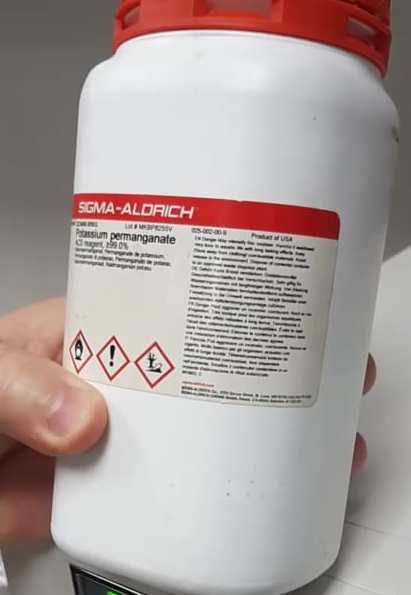
\includegraphics[width=0.3\textwidth]{Tarea1/muestras.png}
    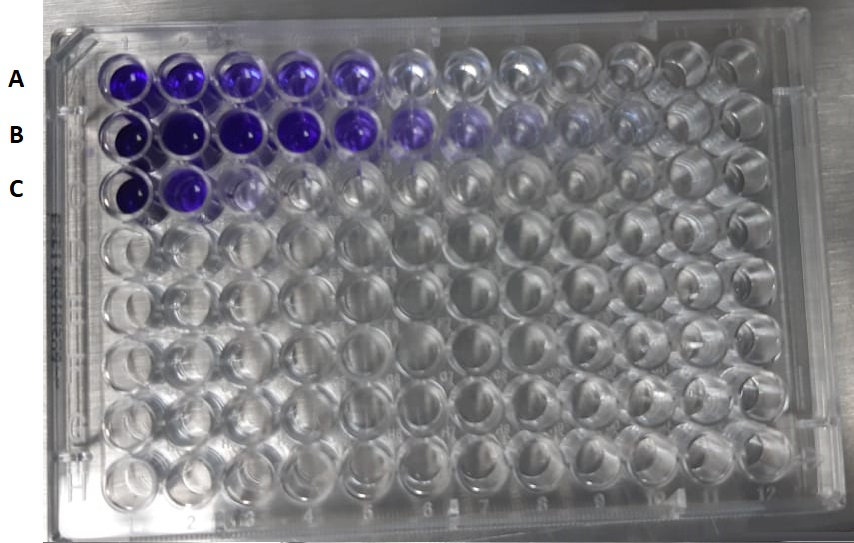
\includegraphics[width=0.49\textwidth]{Tarea2/microplaca2.jpeg}
    \caption{\textbf{Microplaca para el análisis en el espectrofotómetro para mezclas de agua con tinte azul.}}
    \label{microplaca2}
\end{figure}

 %\begin{table}[h!]%[c]{| c |}
%\begin{table}[h!]
    %\centering
\textbf{Tabla 1: Mezcla A.}        

\begin{tabular}{|c|c|c|c|c|c|}
    \hline
    Radio & 1:10 & 1:20 & 1:30 & 1:40 & 1:50\\
    \hline
    Absorbancia & $1.331$ & $0.704$ & $0.450$ & $0.393$ & $0.293$ \\
    \hline\hline\hline
    Radio & 1:200 & 1:500 & 1:1000 & 0:1 & 0:1\\
    \hline
    Absorbancia & $0.083$ & $0.065$ & $0.064$ & $0.050$ & $0.038$\\
    \hline
\end{tabular}
    
\textbf{Tabla 2: Mezcla B.}
    
\begin{tabular}{|c|c|c|c|c|c|}
    \hline
    Radio & 1:2 & 1:4 & 1:8 & 1:16 & 1:32\\
    \hline
    Absorbancia & $3.551$ & $1.820$ & $0.902$ & $0.440$ & $0.229$\\
    \hline\hline\hline
    Radio & 1:64 & 1:128 & 1:256 & 0:512 & \\
    \hline
    Absorbancia & $0.134$ & $0.089$ & $0.074$ & $0.070$ &\\
    \hline
\end{tabular}

\textbf{Tabla 3: Mezcla C.}
    
\begin{tabular}{|c|c|c|c|c|c|}
    \hline
    Radio & 1:10 & $1:10^2$ & $1:10^3$ & $1:10^4$ & $1:10^5$\\
    \hline
    Absorbancia & $0.717$ & $0.106$ & $0.048$ & $0.042$ & $0.045$\\
    \hline\hline\hline
    Radio & $1:10^6$ & $1:10^7$ & $1:10^8$ & $0:10^9$ & \\
    \hline
    Absorbancia & $0.040$ & $0.043$ & $0.037$ & $0.049$ & \\
    \hline
\end{tabular}

    %\caption{\textbf{Primera prueba.}}
    %\label{primera_prueba}
%\end{table}
%\end{table}

\textbf{\textcolor{azul50}{Análisis de los resultados}}

Ya comprobado que los datos fueron obtenidos dentro del rango de limitaciones especificado en la teoría previa, pasamos a procesar en matlab2017b los valores de absorbancia obtenidas por el SkanIt.

Es fácil ver que los valores correspondiente a concentración 0:1 mostrados en la Tabla 1 corresponden al agua destilada sin mezclar con el tinte, valores que dan una medida de error del instrumento ya que este debería estar en $\approx 0.042\pm 0.01$ para $200~\mu l$ mientras que el instrumento da valores con errores máximos visualizados de $\approx\pm 0.09$.

\begin{figure}
    %\centering
    %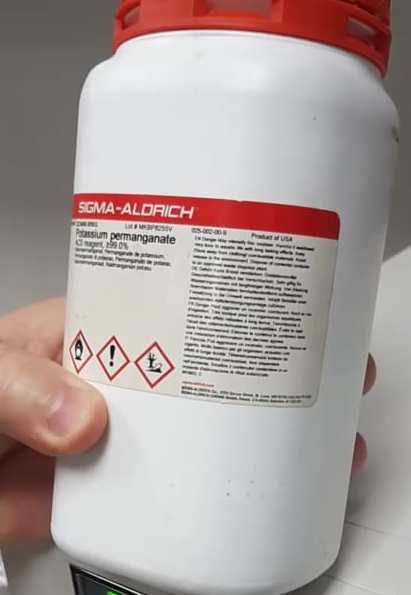
\includegraphics[width=0.3\textwidth]{Tarea1/muestras.png}
    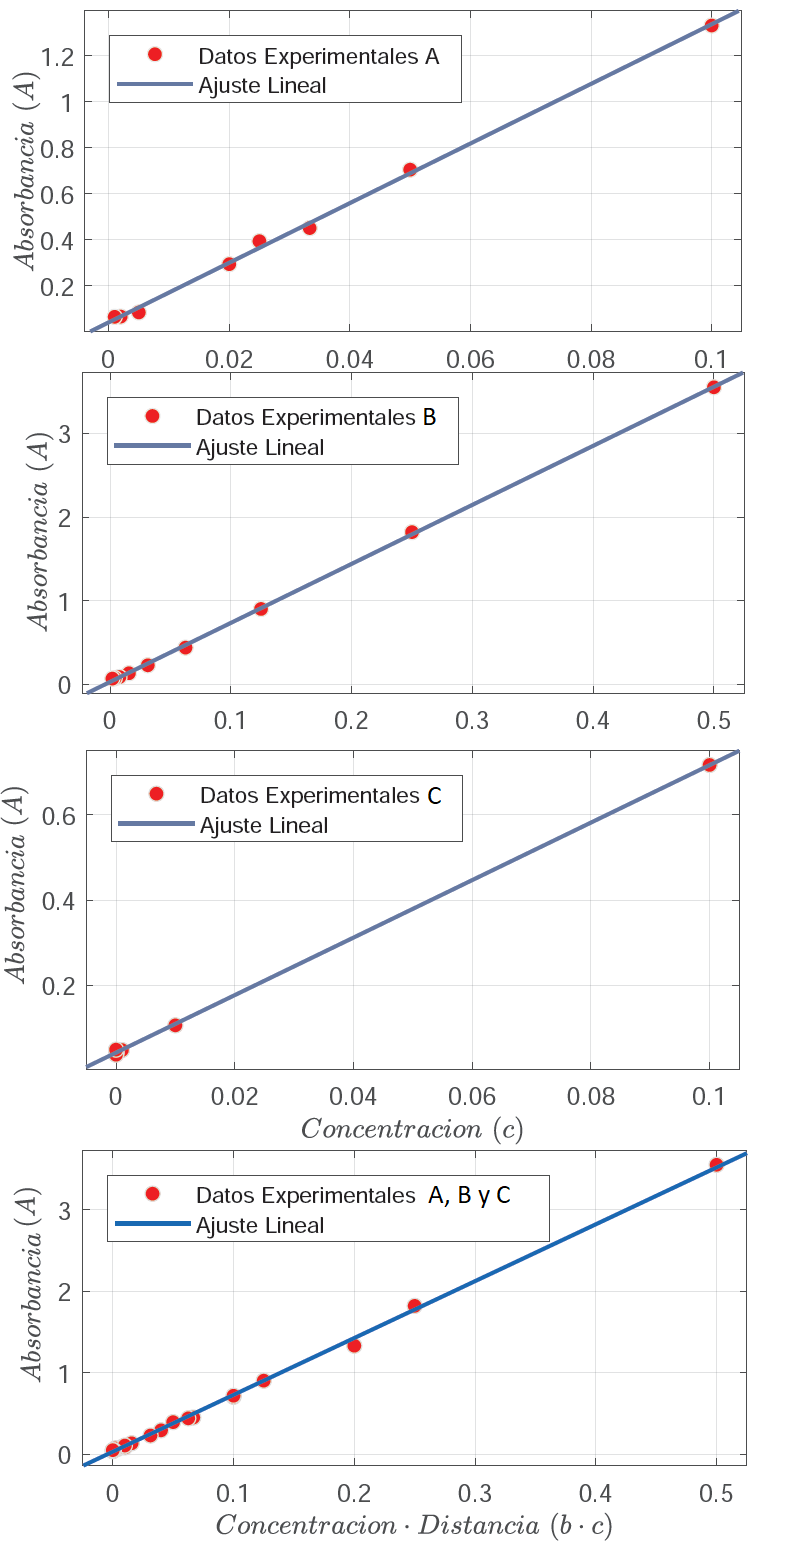
\includegraphics[width=0.49\textwidth]{Tarea2/absorbancia.png}
    \caption{\textbf{Análisis de los resultados de la Tabla 1, 2 y 3.}}
    \label{fig2.1}
\end{figure}

Con los datos mostrados en la Tabla 1, 2 y 3 se procesará a trabajar con los datos en la búsqueda de una tendencia empírica como la predicha por la Ley de Lambert y Beer mostrada en la ec. (\ref{ley}), para esto primeramente se grafeicará la $Absorbancia (A)~ vs~ Concentracion (c)$ y se ajustaran linealmente (a una ecuación de tipo $y~=~a\cdot x$) haciendo uso del Matlab~R2017b~(Ver~Fig.~\ref{fig2.1}).

Como resultado del ajuste lineal de estos datos experimentales tenemos valores de $R-square$ de $\approx 0.9983$, $\approx 0.9997$ y $\approx 0.9997$ para los datos de la Tablas 1, 2 y 3 o las mezclas A, B o C respectivamente, estos valores tan cercarnos a la unidad evidencian la correspondencia predicha por la ec. (\ref{ley}).

Con la intención de generalizar los resultados obtenidos se incluirán todos los mostrados en las Tablas 1, 2 y 3 en un gráfico de Absorbancia (A) vs Concentración $\cdot$ Distancia ($b\cdot c$) como los mostrados en la Fig. \ref{fig2.1}, la distancia del haz monocromático es proporcional a los $\mu l$ finales de las mezclas ($200~\mu l$, $100~\mu l$ y $90~\mu l$ respectivamente). Al realizar el respectivo ajuste lineal resulta en un $R-square \approx 0.9987$ reafirmando también su correspondencia con la ley de de Lambert y Beer.


\textbf{\textcolor{azul50}{Conclusiones}}

Se trabajó con la pipeta de laboratorio para muestras con diferentes proporción entre tinte azul y agua, estás fueron caracterizadas por un espectrofotómetro con un haz de luz monocromático y se comprobó su correspondencia con la Ley de Lambert y Beer, los valores de ajuste obtenidos por el Matlab R2017b comprobarón que el trabajo de laboratorio fue satisfactorio y la manipulación de las pipetas fue la adecuada.


























%\textcolor{azul50}{\textbf{PRACTICA 3: SÍNTESIS Y CARACTERIZACIÓN DE LA ESTABILIDAD DE NANOPARTÌCULAS DE PLATA.}}

%En este laboratorio se introduce al mundo de las nanopartículas con la sintetización de compuestos con plata $AgNPs$ con la intención de evaluar su estabilidad ante diferentes condiciones de pH y concentración de sales, de esta manera completar el estudio de los mismos en el laboratorio.

\textbf{\textcolor{azul50}{Formalismo}}

Las nanotecnologías aprovechan las propiedades excepcionales de partículas que se miden a escalas nanométricas, conocidas comúnmente como nanopartículas.  La nanotecnología se encarga del diseño, producción y empleo de estructuras y objetos a escala nanométrica. Los conocimientos actuales sobre la nanociencia provienen de avances en los campos de la química, física, biología, medicina e ingeniería entre otras. En la ciencia de materiales, las nano partículas permiten la fabricación de productos con propiedades mecánicas nuevas, incluso en termino de superficie de rozamiento, de resistencia al desgaste y de adherencia. En biología y medicina, los nanomateriales se emplean en la mejora del diseño de fármacos y su administración dirigida. En el campo de la electrónica se emplean en el diseño de dispositivos de almacenamiento de datos de menor tamaño, más rápido y con menor consumo de energía. 

A menudo las nanopartículas cuentan con propiedades físicas y químicas muy diferentes a las de los mismos materiales a escala macroscópica. Sus propiedades dependen de su forma y tamaño, características de superficie y estructura interna. La presencia de ciertas sustancias químicas también puede alterar dichas propiedades. Los parámetros principales de las nanopartículas son su forma, el tamaño y la subestructura morfológica de las sustancias. Presentan una suspensión en su mayoría solida en líquidos o una emulsión. En presencia de agentes químicos las propiedades superficiales e interfaciales pueden ser modificadas. Tales agentes pueden estabilizarse contra la coagulación o la agregación conservando la carga de las partículas y modificando su la capa más externa. Dependiendo de la historia de crecimiento y vida útil de una nanopartícula, deben esperarse composiciones muy complejas, en la historia típica de una nanopartícula de combustión, por ejemplo, muchos agentes diferentes son propensos a la condensación de la partícula mientras se enfría y se expone a diferentes ambientes y atmosferas. 

En la nanoescala , las interacciones partícula-partícula están dominadas por fuerzas débiles de Van der Waals, interacciones polares y electrostáticas más fuertes o interacciones covalentes. Dependiendo de la viscosidad y la polarización del fluido, la agregación de partículas está determinada por la interacción entre partículas. Mediante la modificación de la capa superficial, la tendencia de un coloide a coagularse puede aumentar u obstaculizarse. Para las nanopartículas suspendidas en el aire, las cargas pueden acumularse mediante procesos físicos como descarga luminiscente o fotoemisión. En líquidos, carga de partículas. Puede ser estabilizado por procesos electroquímicos en las superficies. Los detalles de las fuerzas de interacción nanopartícula - nanopartícula y las interacciones nanopartícula - fluido son de importancia clave para describir los procesos físicos y químicos, y la evolución temporal de las nanopartículas libres. Siguen siendo difíciles de caracterizar debido a la pequeña cantidad de moléculas. Participa en la capa de superficie activa. Tanto la energía superficial, la carga y la solvatación son parámetros relevantes para considerar. Debido al papel crucial de la interacción nanopartícula - nanopartícula y la interacción nanopartícula - fluido, el término nanopartícula libre puede ser mal interpretado fácilmente. Las fuerzas de interacción ya sean atractivas o repulsivas, determinan crucialmente el destino de las nanopartículas individuales y colectivas. Esta interacción entre nanopartículas que resulta en agregados y / o aglomerados puede influir en su comportamiento. En las suspensiones de gas, la agregación se determina de manera crucial por el tamaño y la difusión, y la coagulación suele ocurrir más rápido que en la fase líquida, ya que el coeficiente de adherencia es más cercano a la unidad que en los líquidos.

Las nanopartículas metálicas han sido de gran interés debido a sus propiedades físicoquímicas, tamaño y comportamiento de los plasmones de superficie, entre las mas usadas encontramos las nanopartículas de plata ($AgNPs$), se han utilizado en diversos ámbitos como la optoelectrónica, biosensores además de otras. Una de las propiedades mas explotada a sido la naturaleza antimicrobiana de la plata. se ha demostrado mediante estudios que la naturaleza microbiana de es dependiente del tamaño y la forma de las nanopartículas, las mas pequeñas tienen una mejor respuesta antimicrobiana. Referente a la forma las nanopartículas con forma esférica se consideran las mas adecuadas para aplicaciones practicas en forma coloidal. 

Con pocas excepciones, la reducción mediada por borohidruro se ha empleado para la síntesis de nanopartículas de plata dispersables. Para nanopartículas de pequeño tamaño, un exceso de agente reductor fuerte, por ejemplo, borohidruro de sodio Se desea (NaBH4), lo que facilita la generación de núcleos instantáneos, lo que resulta en la formación de coloides de plata de tamaño uniforme y monodispersados. Sin embargo, no es fácil obtener nanopartículas de mayor tamaño que empleen la reducción de borohidruro.

Como resultado de un estudio se obtuvieron diferentes muestras obtenidas con diferentes concentración de sus compuestos iniciales, como resultado de esto fueron obteniendos diferentes valores de tamaño medio de las nanopartículas, estos valores medios se relacionaron con los picos en los gráficos de espectrofotometría. 
\begin{figure}
    %\centering
    %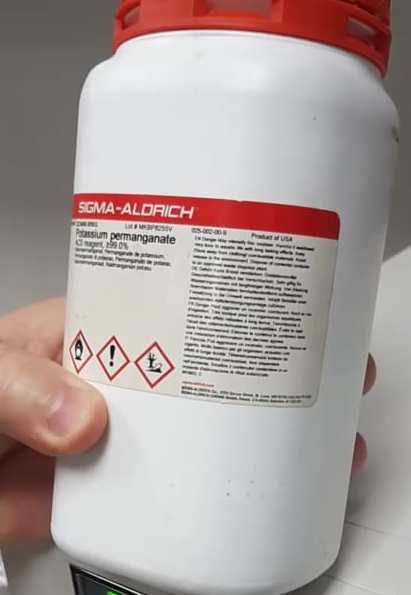
\includegraphics[width=0.3\textwidth]{Tarea1/muestras.png}
    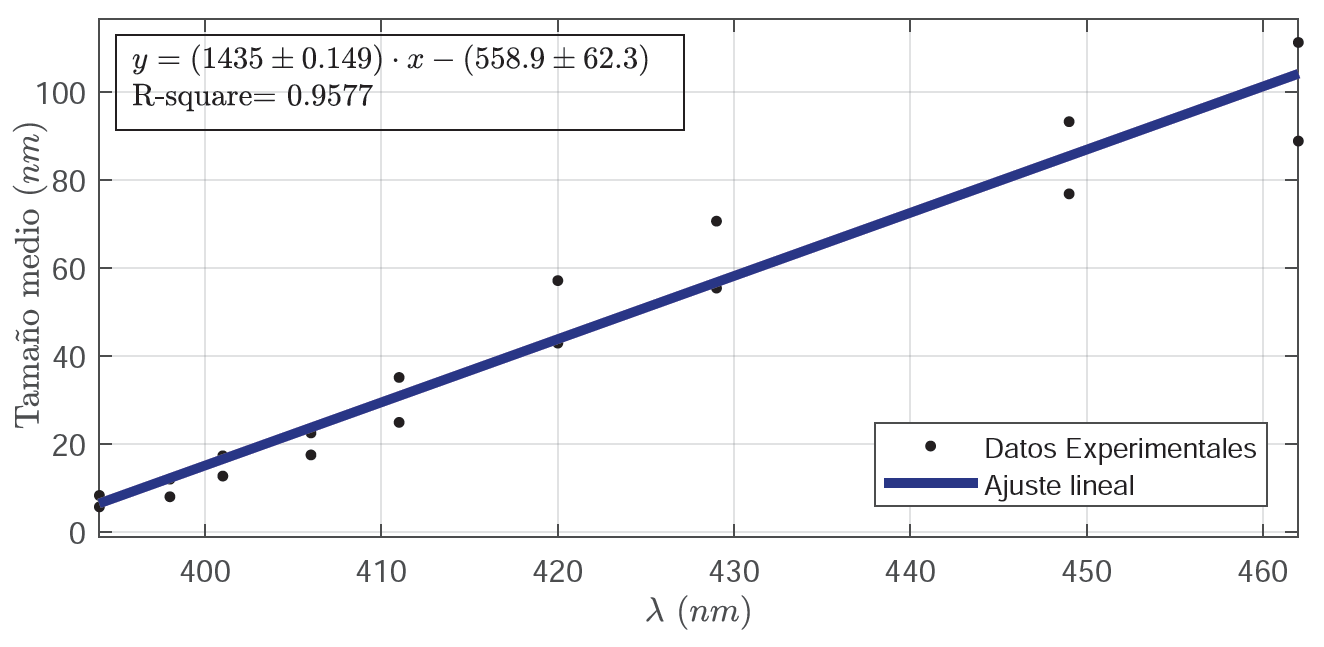
\includegraphics[width=0.49\textwidth]{Tarea3/tamano_experimental.png}
    \caption{\textbf{Ajuste lineal a valores experimentales a $pH=10$.}}
    \label{tamano}
\end{figure}


Ahora, el agente reductor citrato trisódico ($TSC$) contribuye a la formación de nano partículas con una distribución de tamaños mas grandes. También puede dar variación a la variación en la forma de las nanopartículas. Entonces, utilizando cualquiera de los agentes reductores, puede ser difícil sintetizar las nanopartículas de plata, por encima de $50~ nm$ y por debajo de $10~nm$ que tiene una forma bien definida con la monodispersidad deseada. El método de reducción conjunta que emplea dos reductores diferentes (es decir, $NaBH4$ y $TSC$) puede ofrecer un mejor control sobre la nucleación y el crecimiento de las nanopartículas $7,26$. Esto puede ayudar en la síntesis de diferentes tamaños de $AgNPs$ utilizando ligeras variaciones en el mismo protocolo.

\textbf{\textcolor{azul50}{Procedimiento Experimental}}

Aca se presentarán los procedimientos para la obtencion de los compuestos a caracterizar en el laboratorio:

\textbf{Síntesis de nanopartículas de plata.}

Primeramente se realizó la obtención de las nanopartículas de plata, para esto vertemos en un matraz, $250~ml$ de agua que que se agitará continuamente a una temperatura de $\approx 60^o$, agregamos $5~ml$ de trisodio citrato ($Na_3C_6H_5O_7$) con concentración de $0.5~mM$, despues de una espera de $1~min$, agregamos $2~ml$ de nitrato de plata ($AgNO_3$) con concentración de $0.2~mM$, despues de una espera de $5~min$, agregamos $0.5~ml$ de borihidruro de sodio ($NaBH_4$) con concentración de $2~mM$.

\textbf{Estudio de $AgNPs$ para diferentes $pH$.}

Se caracterizarán las nanopartículas de plata $AgNPs$ a diferentes valores de pH, los cambios se realizarán con los compuestos  $NaOH$ y $HCl$, para aumentar y bajar respectivamente el pH de nuestra muestra de nanopartículas, las mediciones de pH se realizarán con el "HI 2210 pH Meter Hanna" (medidor de pH mostrado en la Fig. \ref{ph}). Nuestro objetivo es medir nuestro valor inicial de pH (localizado en la Tabla 4 por una $*$) y obtener 3 muestras para pH mayores y 4 muestras para pH menores, los valores de pH resultantes serán mostrados en la Tabla 4, además, muestras de $200~\mu l$ serán recogidas con las micropipetas correspondiente a cada uno de ellos y puesta en la microplaca para su estudio con un espectrofotómetro como el mostrado en la Fig. \ref{espectro} para un barrido desde $350~nm-650~nm$.

\textbf{Estudio de $AgNPs$ mezcladas en diferentes proporciones con sales de $NaCl$ y $H_2O$.}

Con el objetivo de caracterizar muestra mezcla $AgNPs$ con diferentes concentraciones de sales ($NaCl$) y agua ($H_2O$) se realizarán preparados con porcentajes que varían desde $0\%-100\%$ con un paso de $10\%$, de estos $200~\mu l$ serán recogidas con las micropipetas correspondiente a cada uno de ellos y puesta en la microplaca para su estudio con un espectrofotómetro con barridos desde $350~nm-650~nm$ para la onda monocromática.

\textbf{\textcolor{azul50}{Obtención y análisis de Resultados}}

Se procederá a analizar los datos obtenidos por el espectrofotómetro de los compuestos anteriormente obtenidos.

\textbf{Estudio de $AgNPs$ para diferentes $pH$.}

Se prepararon 8 muestras con diferentes pH, estas obtenidos realizando cambios en la introducción de los compuestos de $NaOH$ y $HCl$, los valores de pH reportados por el "HI 2210 pH Meter Hanna" se muestran en la Tabla 4, estos fueron procesados por el programa matlab2017b y graficados como se muestra en la Fig. \ref{diff_pH}.

\textbf{Tabla 4: Valores de los picos máximo de los gráficos de $Absorbancia~vs~\lambda~(nm)$ en muestras de $AgNPs$ con diferentes $pH$.}

\begin{tabular}{|c|c|c|c|c|}
    \hline
    pH &  2.46 & 6 & 7 & 8 \\
    \hline
    $\lambda(A_{\max})$ & 391 & 397 & 396.6 & 395.8\\
    \hline\hline
    pH & 9.88 $^*$& 11.35 & 11.96 & 12.29\\
    \hline
    $\lambda(A_{\max})$ & 396.5 & 397 & 391 & 390\\
    \hline
\end{tabular}

Al procesar los datos se pudo notar que para los valores extremos $pH~=~2.46$ y $pH~=~12.29$ los gráficos de $A~vs~\lambda ~(nm)$ ya no muestran comportamientos esperados para mezclas con nanopartículas, se podría suponer la destrucción de estás para estos valores extremales. Para los valores intermedios de $pH$ se pudo notar el comportamiento esperado, solo con ligeras variaciones del pico máximo (Ver Figs. \ref{diff_pH})a y \ref{diff_pH})b.

Con la intención de localizar los valores extremos en los gráficos de $A~vs~\lambda ~(nm)~vs~pH$ se presenta la necesidad de encontrar los gráficos de $\partial A/\partial \lambda~vs~\lambda$ para los compuestos con diferentes $pH$ (Ver Fig. \ref{diff_pH}c). La localización se realizó interceptando el gráfico $\partial A/\partial \lambda~vs~\lambda$ con el plano $\partial A/\partial \lambda = 0$ (Ver Fig. \ref{diff_pH}), de está manera se obtuvieron los $\lambda$ para los máximos de absorbancia haciendo uso del matlab2017b, estos fueron introducidos en la Tabla 4 haciéndolos corresponder con sus respectivos $pH$. 

Al analizar estos valores, tenemos que las variaciones de estos valores cumplen con la condición $ \|\overline{ \lambda (A_{\max}) }  - \lambda ( A_{\max})\|~ < ~\Delta\lambda=3 ~nm$  (Error instrumental + Error de simulación = 1 $nm$ + 2 $nm$) los gráficos de $A~vs~\lambda (nm)$ por lo que no es posible diferenciar cambios de los $\lambda$ correspondiente a los picos para los gráficos con diferentes $pH$, de aqui que $\overline{ \lambda ( A_{\max} )} \approx (395.5\pm 3.0)~nm$, según la literatura, los picos correspondientes a este valor se relacionan con el tamaño medio de las nanopartículas (Ver Fig. \ref{tamano}) el cual está dado por 
$\overline{d} \approx  (1.43\pm 0.15)\cdot  \overline{ \lambda ( A_{\max} )} -(559\pm 62)\approx (7.48\pm 0.86)~n m$.

\begin{figure}
    %\centering
    %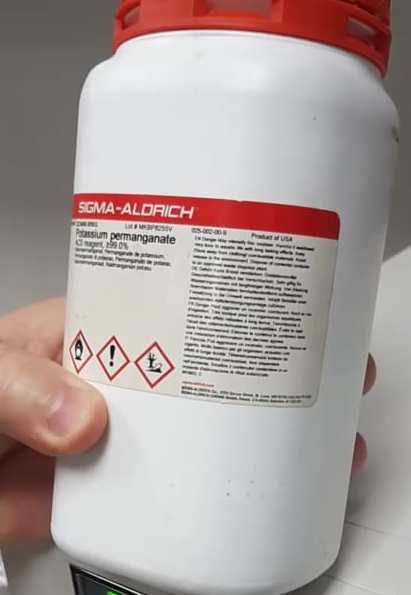
\includegraphics[width=0.3\textwidth]{Tarea1/muestras.png}
    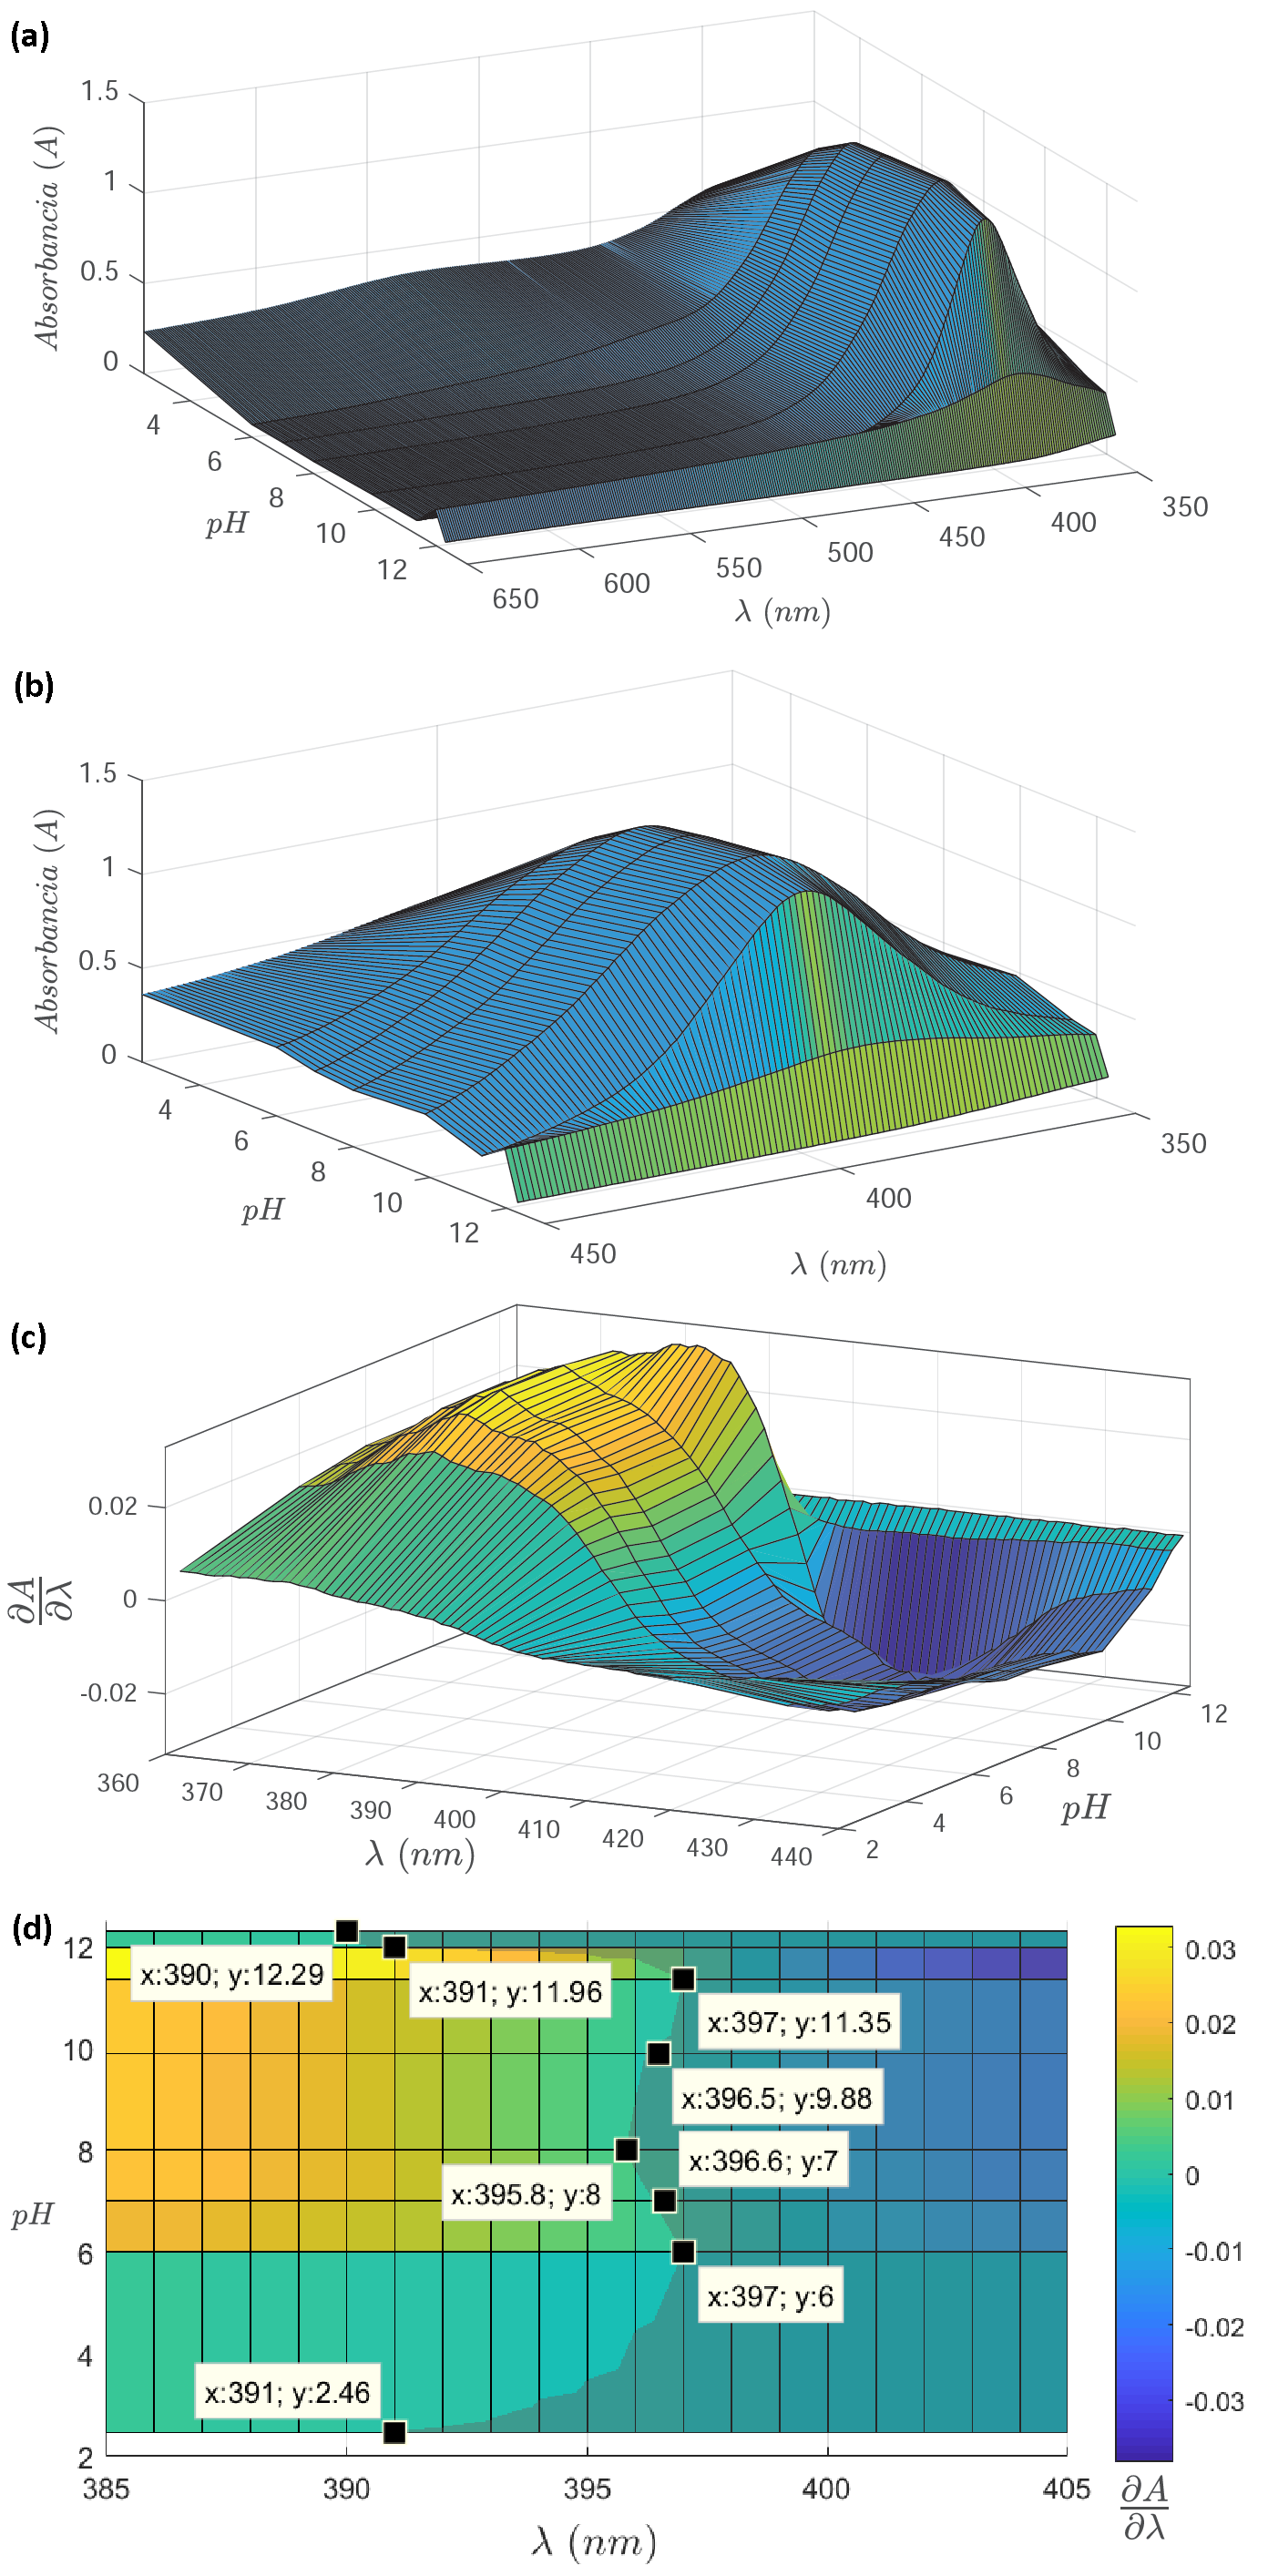
\includegraphics[width=0.49\textwidth]{Tarea3/AgNPs_pH.png}
    \caption{\textbf{Procesamiento de los datos de $AgNPs$ con diferentes $pH$.}}
    \label{diff_pH}
\end{figure}
También en las Figs. \ref{diff_pH}a y \ref{diff_pH}b se puedo apreciar cambios en la altura de esos picos, pero estos cambios no fueron procesados ni serán analizados.

\textbf{Estudio de $AgNPs$ mezcladas en diferentes proporciones con sales de $NaCl$.}

Siguiendo la línea de caracterización en la sección de procedimiento experimental se procesaron los gráficos obtenidos con el espectrofotómetro pero para muestras con diferentes proporciones entre las nanopartículas de plata $AgNPs$ y las sales $NaCl$, las mismas se muestran en las Figs. \ref{nacl}a y \ref{nacl}b. En estas se evidencia la presencia de dos comportamientos superpuestos, típico de la presencia  predominante de dos tamaños medios en nuestra muestra y los mismos se corresponden para todo el barrido caracterizado.

Semejante a los analisis anteriores caracterizaremos los gráficos de $A(\lambda)$ pero a diferentes concentración de $NaCl$, específicamente se procedió a caracterizar los máximos locales de nuestro conjuntos de muestras, para esto se implementó el gráfico relativo a $\partial A/\partial \lambda(\lambda,NaCl)$ (Ver Fig. \ref{nacl}c). El primer grupo de máximos (valores de $\lambda(A_{\max})$) se localizó interceptando el gráfico $\partial A/\partial \lambda(\lambda,NaCl)$ con el plano $\partial A/\partial \lambda =0$, los resultados se muestran en la Tabla 5.

En condiciones normales si tuvieramos la forma matemática específica de los gráficos de $A(\lambda)$ para diferentes muestras de nanopartículas de conocido tamaño podriamos realizar una superposición de los gráficos y encontrar mediante simulación el pico del segundo grupo de nanoparticulas de menos porcentaje de aparición, por cuestiones técnicas y operativas se consideró suficiente solo tener un valor cercano al real de este maximo $\lambda(A_{\max}^2)$, el mismo fue obtenido tratando el gráfico de $\partial^2 A/\partial \lambda^2 (\lambda,NaCl)$ al interceptalo con el plano $\partial^2 A/\partial \lambda^2=0$ en la zona esperada de esta irregularidad (Ver Fig. \ref{nacl}d), los resultados se tabularon en la Tabla 5 haciendolos corresponder son la respectiva proporción del valor de $NaCl$ en muestro compuesto.

\textbf{Tabla 5: Valores de los picos máximo de los gráficos de $Absorbancia~vs~\lambda~(nm)$ en muestras de $AgNPs$ mezcladas con $NaCl$ en diferentes proporciones.}

\begin{tabular}{|c|c|c|c|c|c|}
    \hline
    $NaCl$ &  $0\%$ & $10\%$ & $20\%$ & $30\%$ & $40\%$ \\
    \hline
    $\lambda(A_{\max})$ & $391.5$ & $392$ & $392.2$ & $396.8$ & $392.4$\\
    \hline
    $\lambda(A_{\max}^2)$ & $414.6$ & $414.7$ & $414.6$ & $420.7$ & $414.6$\\
    \hline\hline
    $NaCl$  & $50\%$ & $60\%$ & $70\%$ & $80\%$ & $90\%$ \\
    \hline
    $\lambda(A_{\max})$ & $391.9$ & $391.8$ & $392.9$ & $392.6$ & $393$\\
    \hline
    $\lambda(A_{\max}^2)$ & $414.6$ & $414$ & $416.9$ & $417.5$ & $421$\\
    \hline
\end{tabular}

Al analizar los datos de la Tabla 5, tenemos un caso atípico para una proporción del $30\%$ para el $NaCl$, tanto para los resultados de $\lambda (A_{\max})$ y $\lambda (A_{\max}^2)$, dado la poca cantidad de casos presentados y la no correspondencia con el resto de los valores solo podemos asumir que sea un error humano en algún momento de implementado el procedimiento de caracterización, y que como resultado se haya contaminado el compuesto, por lo cual desechamos este gráfico para los análisis siguientes.

\begin{figure}
    %\centering
    %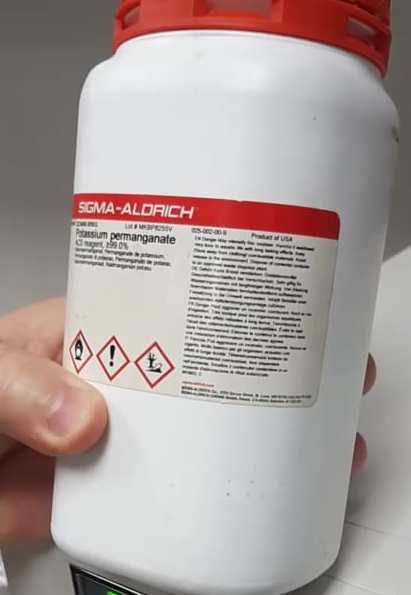
\includegraphics[width=0.3\textwidth]{Tarea1/muestras.png}
    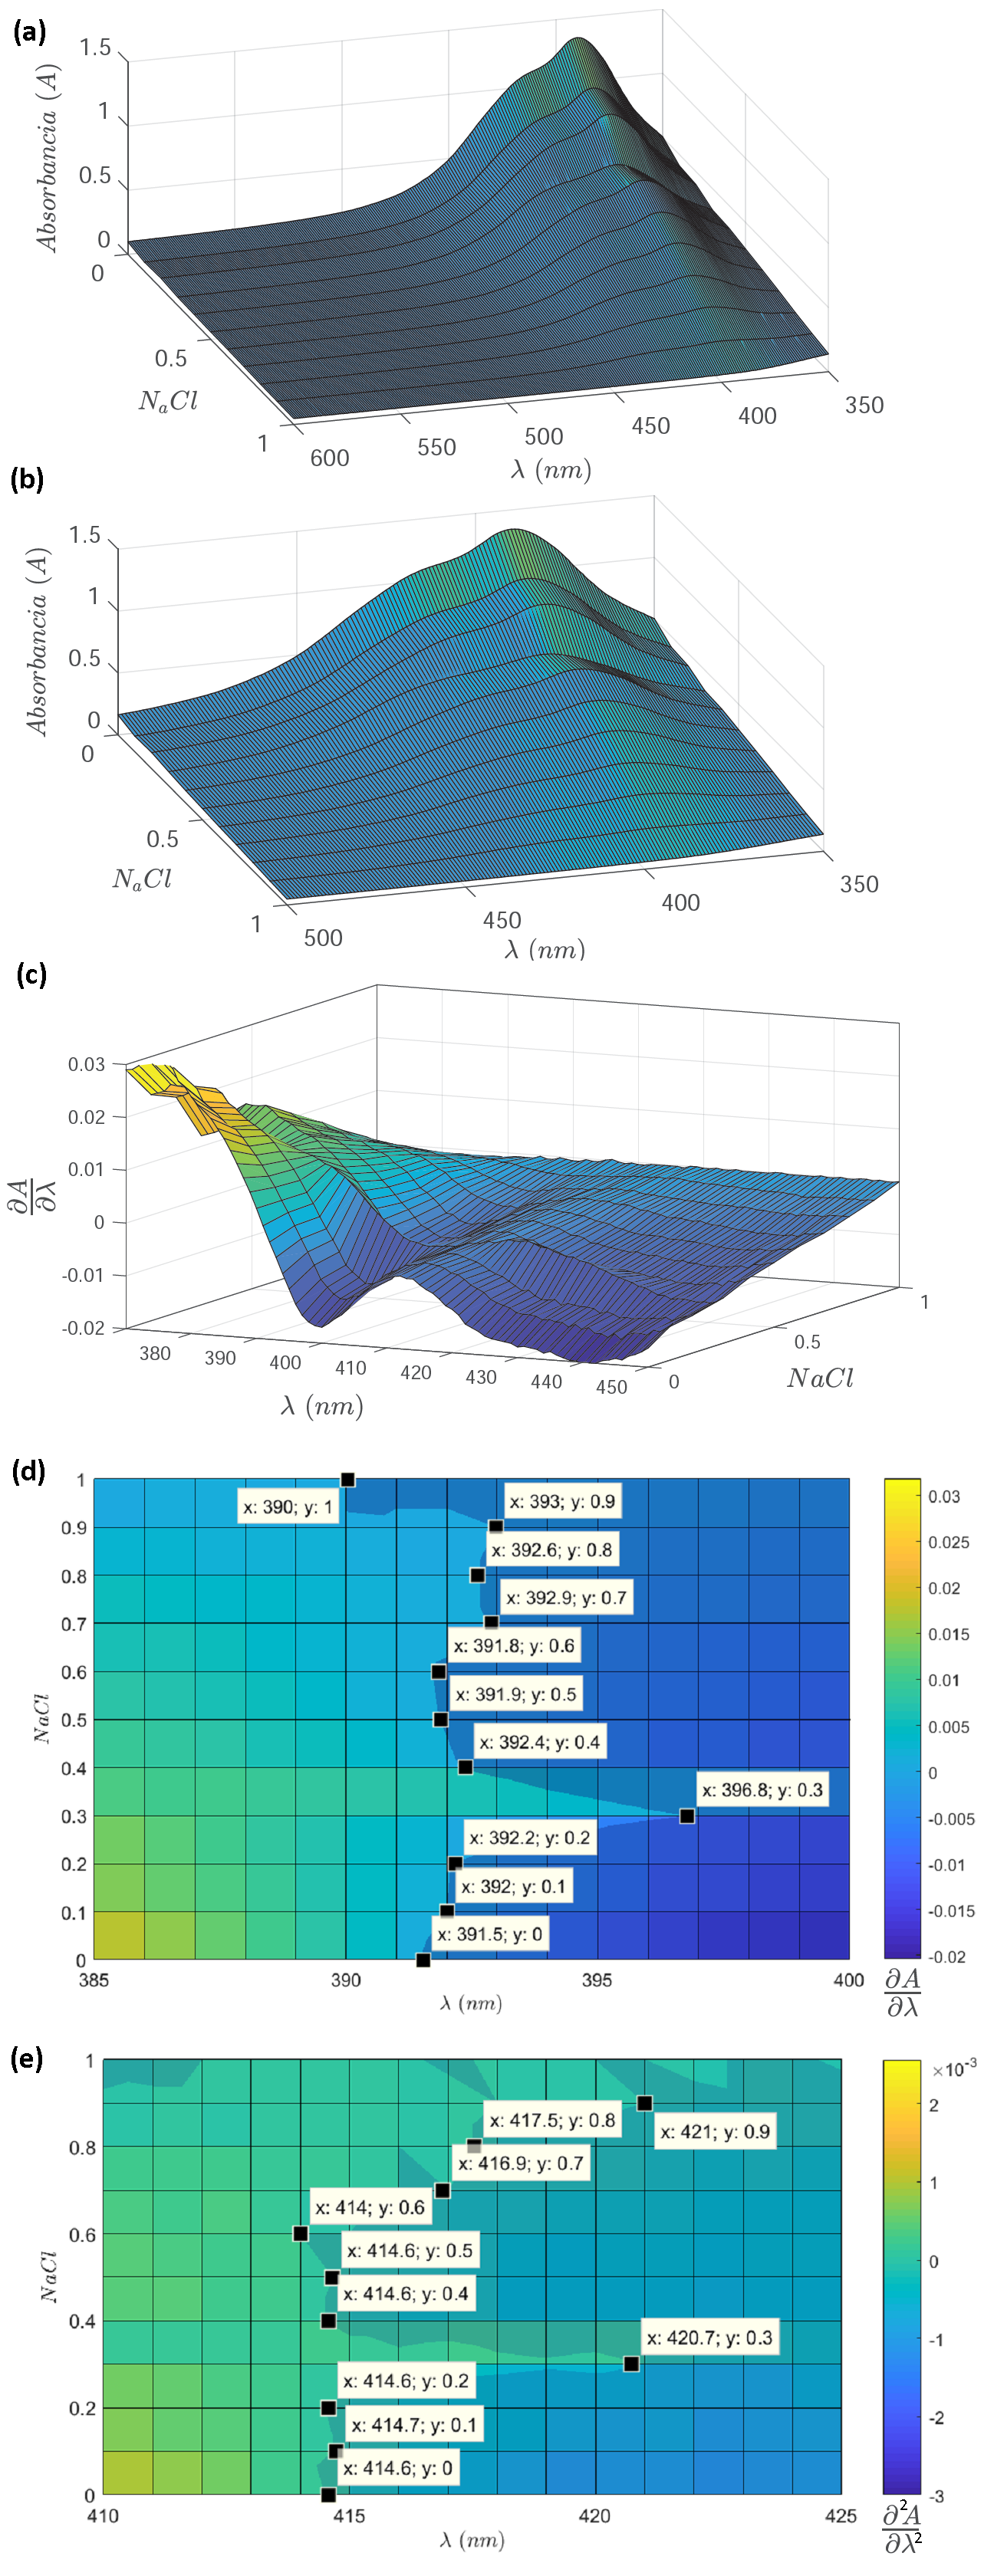
\includegraphics[width=0.47\textwidth]{Tarea3/AgNPs_NaCl.png}
    \caption{\textbf{Procesamiento de los datos de $AgNPs$ con diferentes concentración de $NaCl$.}}
    \label{nacl}
\end{figure}

Exceptuando al correspondiente caso atípico, tenemos que las variaciones de estos valores cumplen con la condición $ \|\overline{ \lambda (A_{\max}) }  - \lambda ( A_{\max})\|~ < ~\Delta\lambda=3 ~nm$  (Error instrumental + Error de simulación = 1 $nm$ + 2 $nm$) y que $ \|\overline{ \lambda (A_{\max}^2) }  - \lambda ( A_{\max}^2)\|~ < ~\Delta\lambda=4 ~nm$  (Error instrumental + Error de simulación = 1 $nm$ + 3 $nm$), el aumento del error de simulación está relacionado con los filtros que se aplicaron para procesar los datos en el programa matlab2017b, estos aumentan la incertidumbre de los resultados a obtener.

Al visualizar los resultados de $\lambda (A_{\max})$ y $\lambda (A_{\max}^2)$ obtenidos de los gráficos de $A~vs~\lambda (nm)$ se visualizaron cambios menores a los errores de nuestros datos por lo que no es posible diferenciar cambios de los $\lambda$ correspondiente a los picos principales buscados, de aqui que $\overline{ \lambda ( A_{\max} )} \approx (392.3\pm 3.0)~nm$, $\overline{ \lambda ( A_{\max}^2 )} \approx (415.8\pm 4.0)~nm$.

Haciendo uso de los resultados mostrados en la literatura, los picos correspondientes a los valores $\overline{ \lambda ( A_{\max} )}$ y $\overline{ \lambda ( A_{\max}^2)}$ se relacionan con el tamaño medio de las nanopartículas (Ver Fig. \ref{tamano}), los cuales están dados por:

$\overline{d} \approx  (1.43\pm 0.15)\cdot  \overline{ \lambda ( A_{\max} )} -(559\pm 62)\approx (3.6\pm 0.46)~n m$ 

$\overline{d_2} \approx  (1.43\pm 0.15)\cdot  \overline{ \lambda ( A_{\max}^2)} -(559\pm 62)\approx (37.2\pm 5.4)~n m$.

\textbf{Estudio de $AgNPs$ mezcladas en diferentes proporciones con sales de $H_2O$.}

Realizando un análisis semejante a los compuestos con sales se procesarán los gráficos obtenidos con el espectrofotómetro pero para muestras con diferentes proporciones entre las nanopartículas de plata $AgNPs$ y agua $H_2O$, las mismas se muestran en las Figs. \ref{h2o}a y \ref{h2o}b. En estas se evidencia la presencia de comportamiento típico de nanopartículas para concentraciones de agua de $\leq 30\%$, en caso contrario en los gráficos no se identifica los mismos y se asume la destrución de las nanopartículas para esas concentraciones, estos gráficos no serán procesados en la caracterización siguiente.

Se caracterizarán los gráficos de $A~vs~\lambda ~(nm)$ pero a diferentes concentración de $H_2O$, específicamente se procedió a caracterizar los máximos locales de nuestro conjuntos de muestras, para esto se implementó el gráfico relativo a $\partial A/\partial \lambda~vs~\lambda~vs~H_2O$ (Ver Fig. \ref{h2o}c). Los máximos (valores de $\lambda(A_{\max})$) se localizarón con la intercepción del gráfico $\partial A/\partial \lambda~vs~\lambda~vs~H_2O$ con el plano $\partial A/\partial \lambda =0$ (Ver Fig. \ref{h2o}d), los resultados se muestran en la Tabla 6.

\textbf{Tabla 6: Valores de los picos máximo de los gráficos de $Absorbancia~vs~\lambda~(nm)$ en muestras de $AgNPs$ mezcladas con $H_2O$ en diferentes proporciones.}

\begin{tabular}{|c|c|c|c|c|c|}
    \hline
    $H_2O$ &  $0\%$ & $10\%$ & $20\%$ & $30\%$ \\
    \hline
    $\lambda(A_{\max})$ & $392.1$ & $395.3$ & $396$ & $395$\\
    \hline
\end{tabular}

Al comparar los resultados obtenidos se notan diferencias marcadas con las muestras mezcladas con sales $NaCl$, para las muestras con agua no se mostraron evidencia de un segundo grupo de partículas, pero si de la traslación del pico principal de absorción a valores de $\lambda$ mayores cuando se comparan los resultados de $\lambda(A_{\max})$ para $H_2O$ a $0\%$ y los compuestos con agua ($H_2O$ a $>0\%$).

Al analizar los datos de la Tabla 5, se muestran que los resultados para $\lambda (A_{\max})$ son pocos, por lo que no es posible hacer una correspondencia entre ellos. Además, no se evidencia cambio en la posición de los picos, para los compuestos con agua $H_2O>0\%$ ya que tenemos que las variaciones de estos valores cumplen con la condición $ \|\overline{ \lambda (A_{\max}) }  - \lambda ( A_{\max})\|~ < ~\Delta\lambda=3 ~nm$  (Error instrumental + Error de simulación = 1 $nm$ + 2 $nm$), de aqui que se tratará con los valores medios $\overline{ \lambda ( A_{\max} )} \approx (395.4\pm 3.0)~nm$. 

\begin{figure}
    %\centering
    %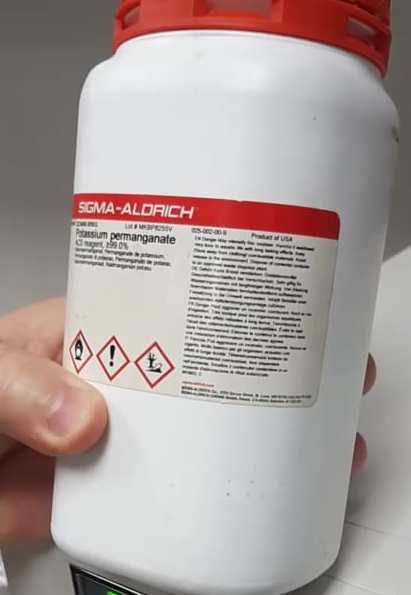
\includegraphics[width=0.3\textwidth]{Tarea1/muestras.png}
    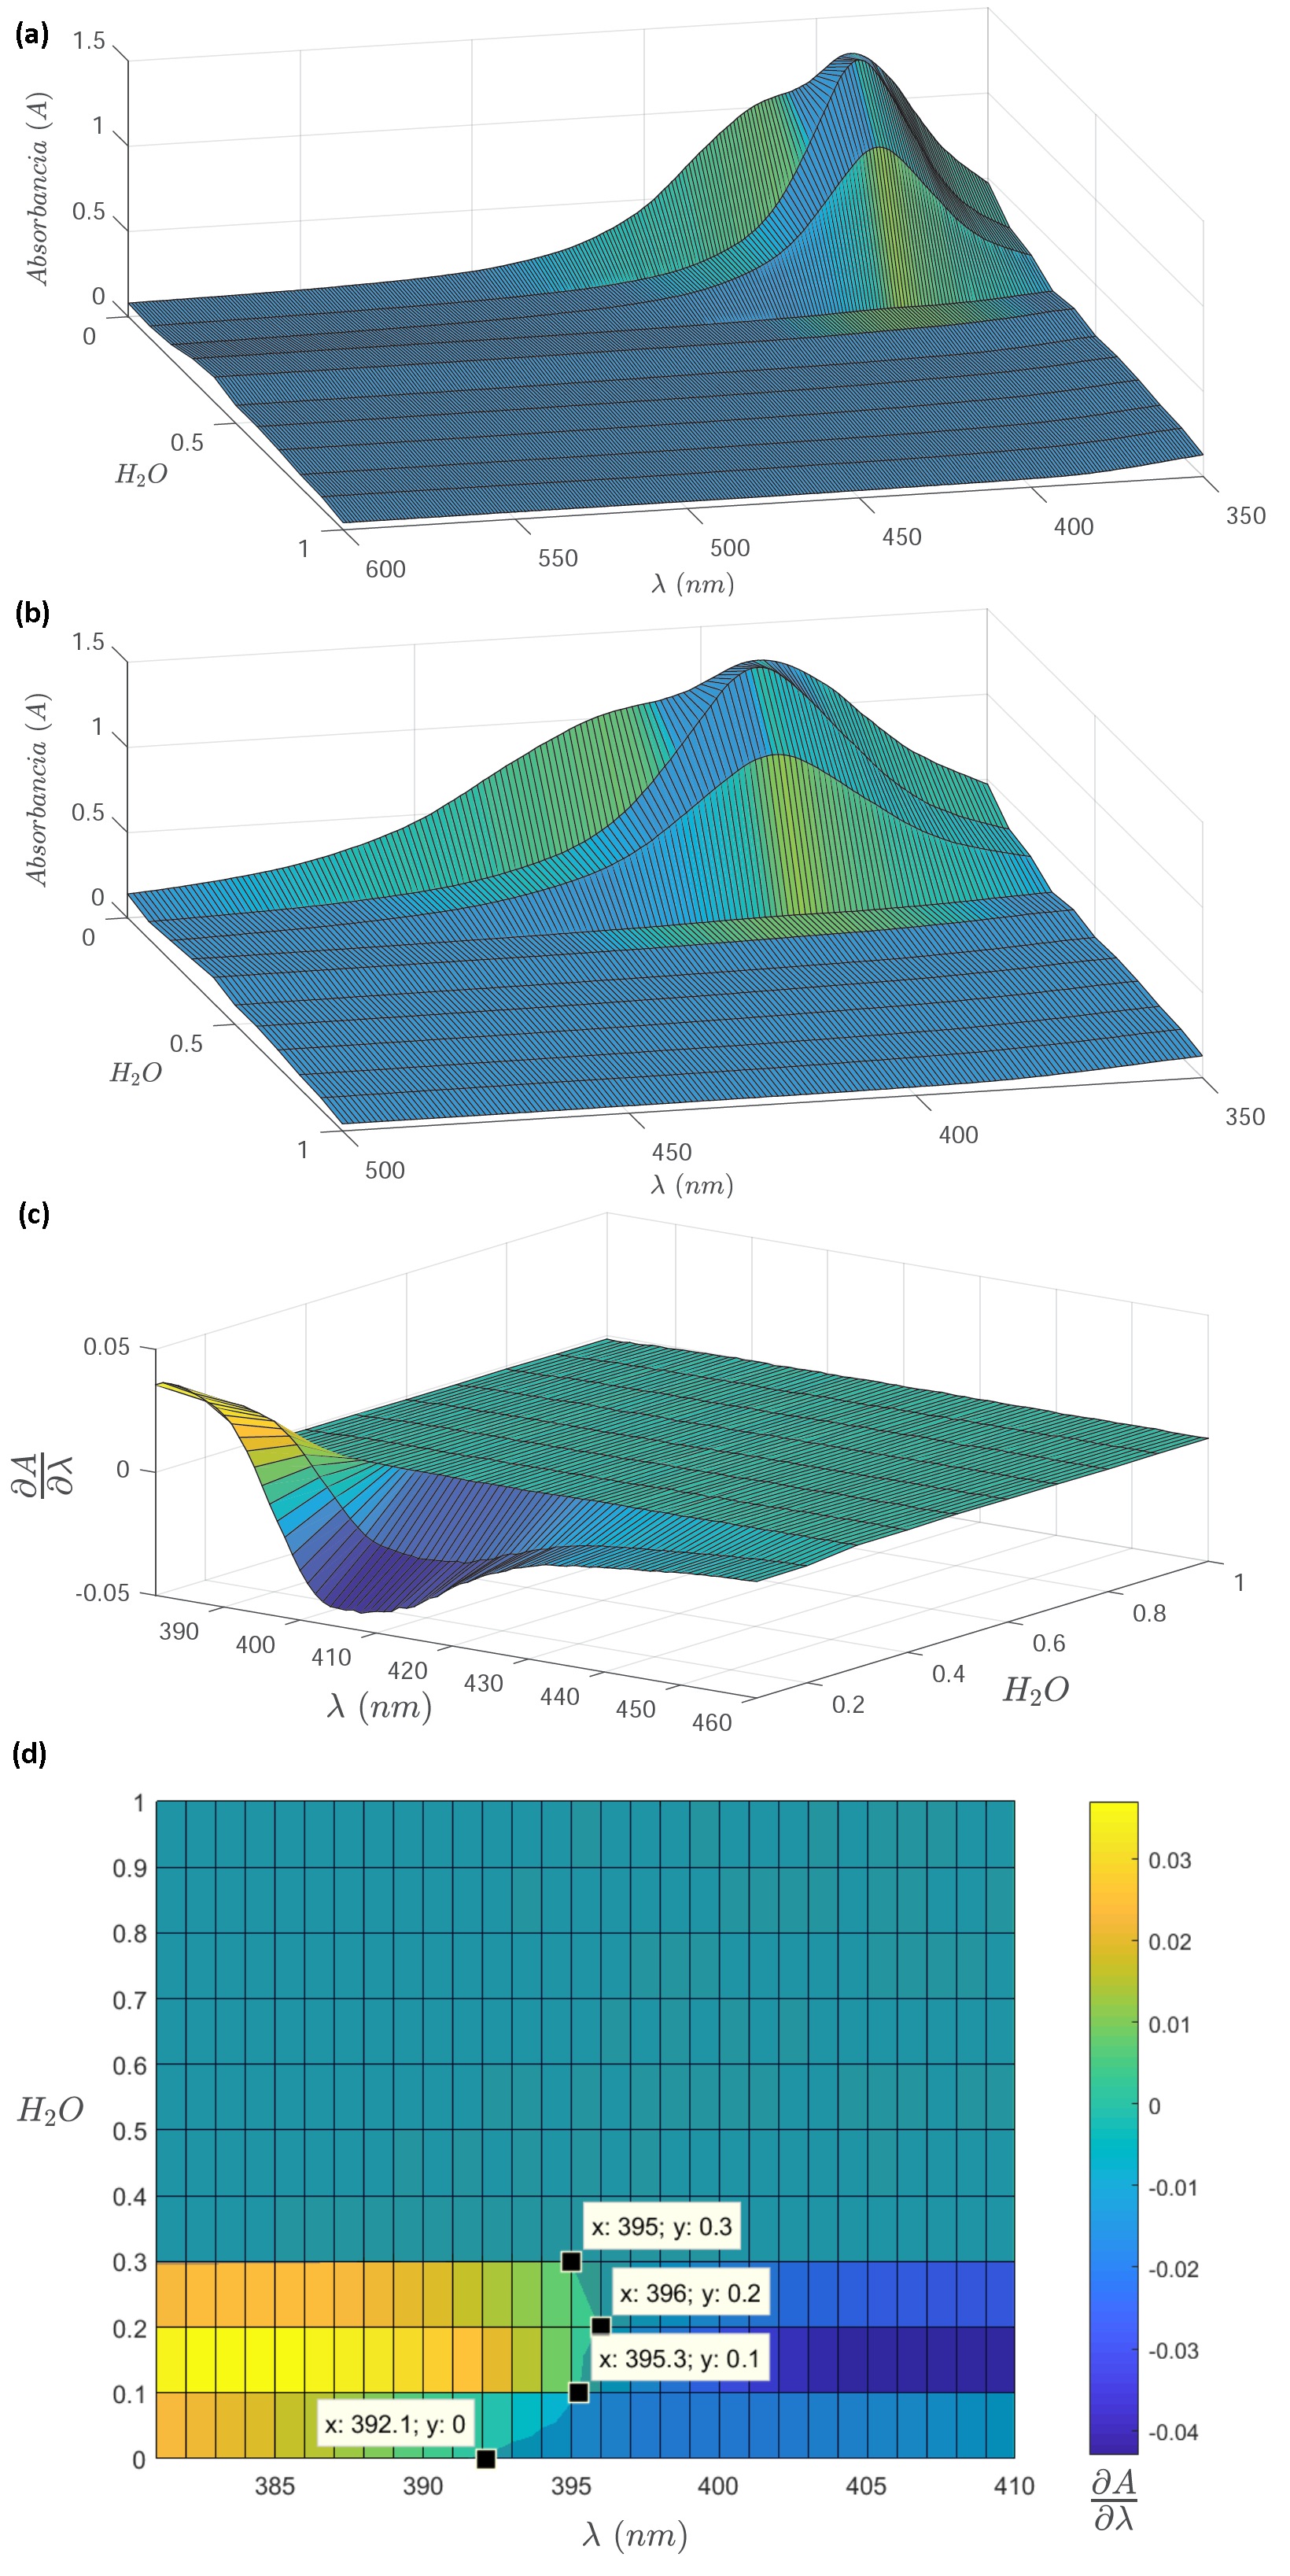
\includegraphics[width=0.49\textwidth]{Tarea3/AgNPs_H2O.png}
    \caption{\textbf{Procesamiento de los datos de $AgNPs$ con diferentes concentración de $H_2O$.}}
    \label{h2o}
\end{figure}

Haciendo uso de los resultados mostrados en la literatura, los picos correspondientes a los valores $\overline{ \lambda ( A_{\max} )}$ se relacionan con el tamaño medio de las nanopartículas (Ver Fig. \ref{tamano}), por lo cual podemos suponer que poseemos nanopartículas con tamaño medio de:

$\overline{d} \approx  (1.43\pm 0.15)\cdot  \overline{ \lambda ( A_{\max} )} -(559\pm 62)\approx (8.05\pm 0.91)~n m$

\textbf{\textcolor{azul50}{Conclusiones}}

En este laboratorio se trabajaron compuestos de nanopartículas de plata $AgNPs$, en los mismos se logró evaluar la estabilidad de nuestro compuesto ante diferentes condiciones de $pH$, o al ser mezclado con $NaCl$ y $H_2O$, se logró encontrar un valor aproximado de los valores de tamaño de grano para cada uno de nuestros compuestos y pudimos comprobar la diferencia en estos valores. Con el análisis de nuestros datos se da por cumplido la pláctica.







%\textcolor{azul50}{\textbf{PRÁCTICA 4: PRINCIPIO Y APLICACIONES DE LA MICROSCOPÍA DE FUERZA ATÓMICA.}}

%En este laboratorio se busca analizar una muestra sanguínea mediante la técnica de AFM, y con los resultados conocer la morfología de las células conocidas como glóbulos rojos (eritrocitos).

\textbf{\textcolor{azul50}{Formalismo}}

La aplicación de un microscopio de fuerza atómica (AFM) para los trabajos en labratorio  ha proporcionado aumentar significativamente los conocimientos sobre las estructuras y procesos celulares. Este es un instrumento mecano-óptico capaz de detectar fuerzas del orden de los nanonewtons, el mismo es capaz de registrar continuamente su topografía mediante una sonda o punta afilada de forma piramidal o cónica, la sonda va acoplada a un listón o palanca microscópica muy flexible de sólo unos $200~\mu m$. El microscopio de fuerza atómica ha sido esencial en el desarrollo de la nanotecnología, para la caracterización y visualización de muestras a dimensiones nanométricas.

El AFM es una técnica tradicionalmente usada para mapear la topografía y estudiar las propiedades de materiales a escalas nanometricas, en esta se usa una punta tipo aguja en un extremo del cantilever para interactuar con el material (muestra). La interacción entre las muestras y la punta se manifiesta en fuerzas atractivas o repulsivas. Estas fuerzas brindan información sobre la topografía de la muestra. Si la punta y la muestra están cerca una de la otra, la fuerza de atracción trae la punta hacia la muestra, y cuando la punta es puesta en contacto con la muestra, la fuerza de repulsión rechaza a la punta lejos de la muestra. Este fenómeno puede ser
explicado por el principio de exclusión de Pauli. El cantilever actúa como el sensor de fuerza. Los cantilevers vienen en diferentes formas, la selección depende en el tipo de medición a la que será destinado. Con objeto de tener una sensibilidad pequeña a la fuerza, la masa del cantilever debe ser pequeña.

La aplicación del programa XEI para analizadar muestras proporcionadas por un equipo AFM es una práctica habitual ya que posee herramientas fáciles de usar y dinámicas para el procesamiento de imágenes, el análisis cualitativo y cuantitativo,
estadística, exportación e impresión de imágenes procesadas y resultados de las mediciones realizadas a las células sanguíneas, por eso es la herramienta que tradicionalmente se utiliza para ello por los investigadores ya que se convierte en la actualidad en una necesidad la caracterización de un
material con sus propiedades como las eléctricas,
mecánicas y químicas a escala nanométricas y de esta manera entender la naturaleza del
material.

La implementación de esta técnica en la investigación de los eritrocitos se considera algo habitual en el mundo científico, dadas las características de las células y lo munerosas que son en la sangre, mediante está técnica se ha podido constatar que los eritrocitos de los mamíferos, carecen de núcleo y de mitocondrias, además normalmente presentan forma oval, con una depresión en el centro mostrandose con una membrana con un espesor menor
a $0.1\%$ de la célula.

\textbf{\textcolor{azul50}{Procedimiento experimental}}

La muestra a estudiar fue el resultado de una extracción de sangre por medio de venopunción de un paciente, una gota de la misma fue colocada sobre una placa de vidrio  y una vez que se asegura que se distribuya de manera laminal a lo largo de la placa, se deja secar la misma por un tiempo aproximado de $10~min$, se procede entonces a la obtención de imagenes de los eritrocitos por AFM para su posterior análisis con XEI y matlab como programa alternativo para comparar resultados.

\textbf{Procesamiento con XEI y con matlab}

Para su procesamiento se hace necesario primeramente homogeneizar el fondo de la imagen, se sigue con la deteción de granos en la imagen, y obtención de los perfiles de superficies de cada grano detectado. Ya logrado esto se pasa a obtener las respectivas distribuciones correspondientes a los parámetros de células (diámetro medio $\overline{d}$ (considerandolos circulares), área de la superficie superior ($A$), perímetro de la célula en su vista superior ($P$), volumen total ($V$), valores de rugosidad superficial ($R_{vp}$ y $R_{rms}$), estos se visualizarán mediante sus respectivos histogramas. Finalmente se procederá a calcular los valores medio de estos parámetros con sus valores medios.

Se comparan los resultados obtenidos de forma independiente, valorando las fortalezas de cada estudio de forma independiente.

\textbf{\textcolor{azul50}{Obtención y análisis de Resultados}}

Se  procederá  a  analizar dos perfiles (ver Fig. \ref{original}) obtenidos al aplicar la técnica de AFM sobre una misma muestra.
\begin{figure}
    \centering
    %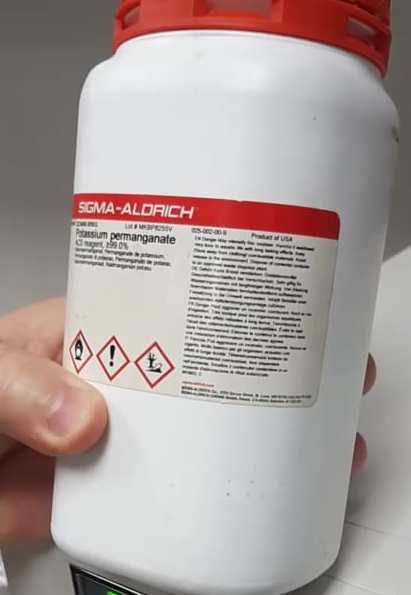
\includegraphics[width=0.3\textwidth]{Tarea1/muestras.png}
    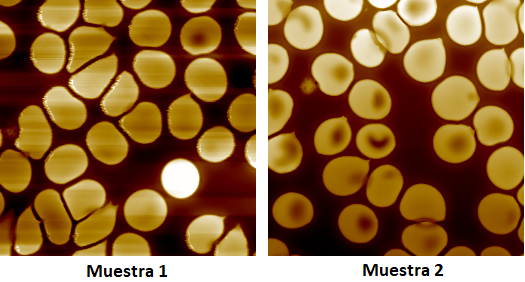
\includegraphics[width=0.49\textwidth]{Tarea4/muestras_originales.png}
    \caption{\textbf{Imagenes .tiff obtenidos con AFM.}}
    \label{original}
\end{figure}
Se utilizaron los programas XEI y matlab para procesar los perfiles, la renderización de los mismos se muestra en la Fig. \ref{perfil} mostrando claramente la presencia de elementos celulares bien definidos.
\begin{figure}
    \centering
    %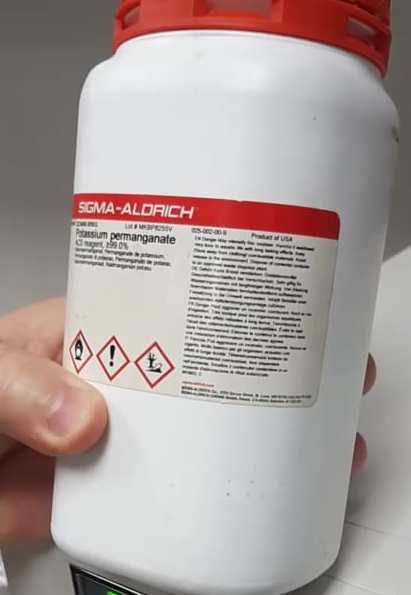
\includegraphics[width=0.3\textwidth]{Tarea1/muestras.png}
    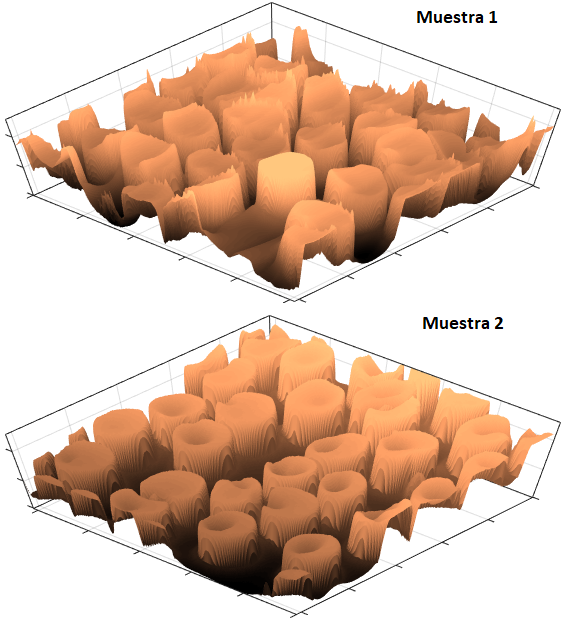
\includegraphics[width=0.49\textwidth]{Tarea4/perfil.png}
    \caption{\textbf{Gráficos 3D realizado en matlab de las muestras tratadas.}}
    \label{perfil}
\end{figure}
Se procedió inicialmente a homogeneizar la superficie de la muestra, este proceso es prácticamente automático con el XEI, pero en el caso del matlab se tuvo que primeramente recurrir por un proceso iterativo permitiendo mejorar significativamente el perfil resultante al despreciar las irregularidades superficiales del medio.
\textbf{\begin{figure}
    \centering
    %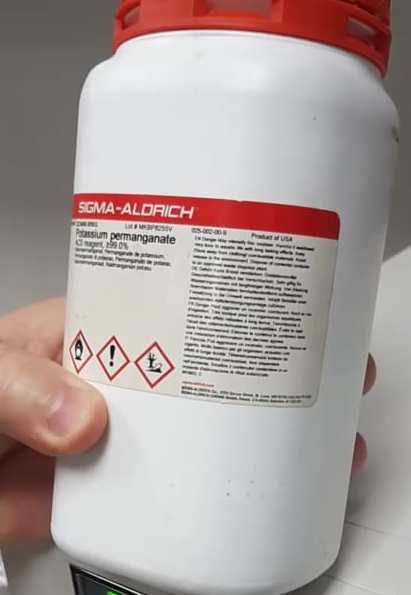
\includegraphics[width=0.3\textwidth]{Tarea1/muestras.png}
    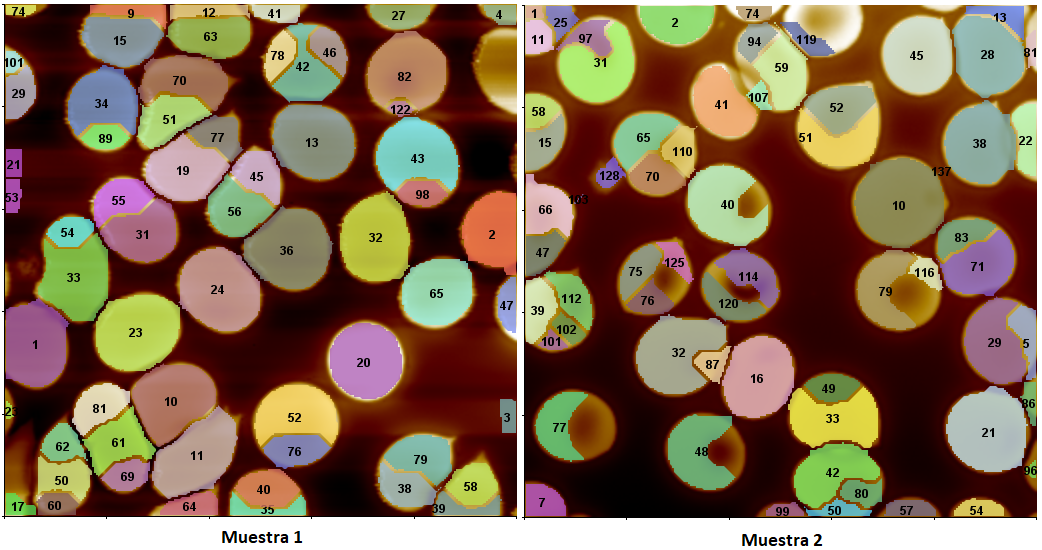
\includegraphics[width=0.49\textwidth]{Tarea4/XEI.png}
    \caption{\textbf{Procesamiento y localización de las objetos con XEI.}}
    \label{xei}
\end{figure}}
La identificación de los elementos en los perfiles se realiza de forma automática con el XEI (ver Fig. \ref{xei}), este identifica correctamente abruptos de gradiente en la imagen, como resultado de esto se localizarón efectivamente 229 elementos en las dos muestras mediante este programa, los errores posiblemente sean debido a una calibración errónea de los parámetros en el software introducidos por el usuario, esto disminuirá la fiabilidad de los resultados esperados. Para la identifiación de objetos realizado por el matlab se procedió con el aumento de contraste, la binarización y la identificación de objetos con redes neuronales (ver Fig. \ref{tratamiento}), se localizaron efectivamente 72 elementos, los resultados se muestran muy acordes con la comparación visual realizada a los perfiles originales.
\begin{figure}
    \centering
    %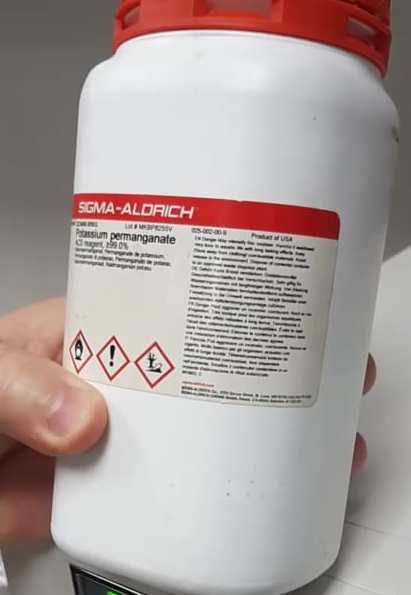
\includegraphics[width=0.3\textwidth]{Tarea1/muestras.png}
    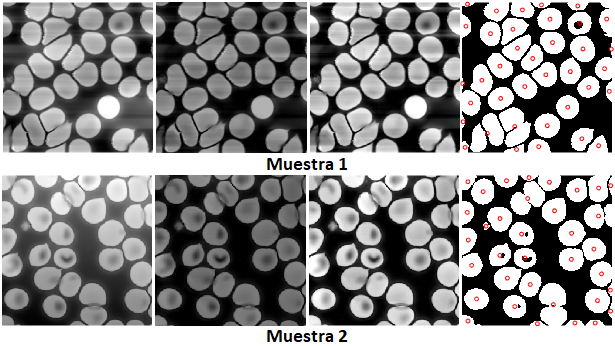
\includegraphics[width=0.49\textwidth]{Tarea4/tratamiento.png}
    \caption{\textbf{Procesamiento y localización de las objetos con matlab.}}
    \label{tratamiento}
\end{figure}
Se procede a la obtención de los parámetros celulares de interés ya explicados en la sección de procedimiento esperimental, la distribución de los mismos es visualizable en la Fig. \ref{histogramaprogram} para los resultados mostrados por XEI, y para el caso del matlab se procedió a la agrupación de parámetros correspondientes a las dos muestras, los mismos son mostrados en la Fig. \ref{histograma1}. 
\textbf{\begin{figure}
    \centering
    %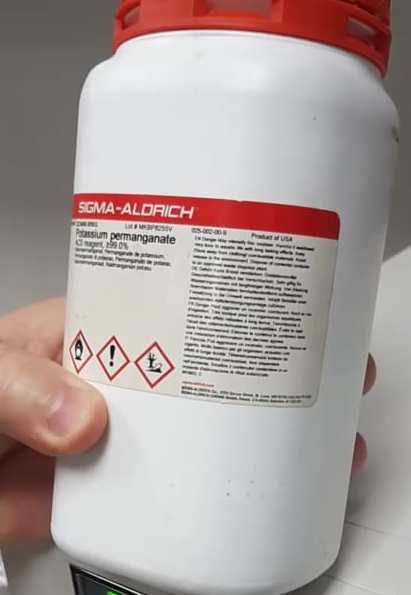
\includegraphics[width=0.3\textwidth]{Tarea1/muestras.png}
    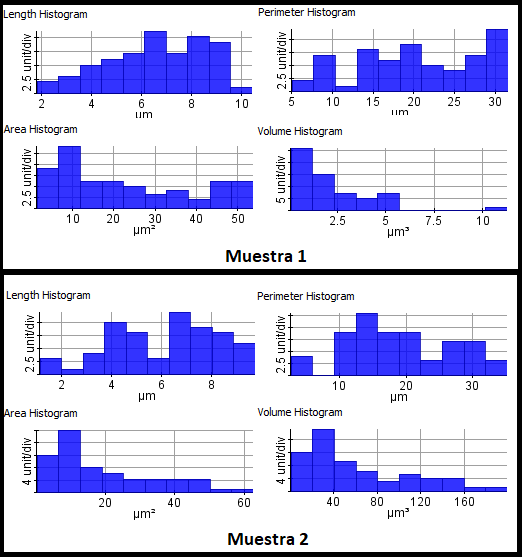
\includegraphics[width=0.49\textwidth]{Tarea4/histogramaprogram.png}
    \caption{\textbf{Histogramas de parámetros calculados por XEI.}}
    \label{histogramaprogram}
\end{figure}}
Al comparar la forma de las distribuciones se pudo constatar que hay correspondencia en los datos procesados por el XEI, pero las comparaciones con las distribuciones obtenidas con matlab muestra formas y agrupamientos inesperados, en especial en los parámetros correspondientes al área ($A$), volumen ($V$) y perímetro ($P$). Finalmente los párametros obtenidos se muestran en la Tabla 7.

\textbf{\begin{figure}
    \centering
    %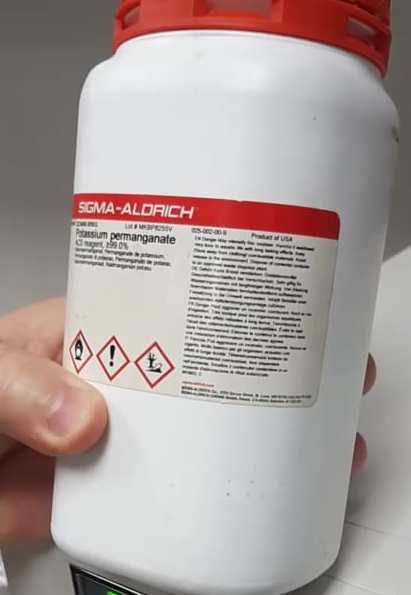
\includegraphics[width=0.3\textwidth]{Tarea1/muestras.png}
    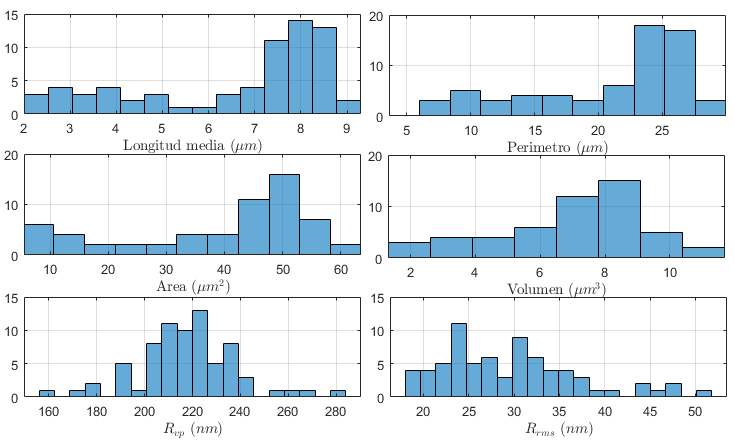
\includegraphics[width=0.49\textwidth]{Tarea4/histograma1.png}
    \caption{\textbf{Histogramas de parámetros calculados por matlab.}}
    \label{histograma1}
\end{figure}}
 
 \textbf{Tabla 7: Valores de los parámetros obtenidos al analizar las celulas con AFM.}
 
 \begin{tabular}{|c|c|c|c|}
    \hline
    Símbolo & XEI (media) & Matlab\\
    \hline
     $\overline{d}$ ($~\mu m$)& $6.584\pm 2.02$ & $6.88\pm 1.72$\\
     \hline
    $P$  ($\mu m$)& $20.36 \pm 7.466$ & $22.89\pm 9.04$  \\
     \hline
     $A$ ($\mu m^2$)& $22.48\pm 15.83$ &  $38.06\pm 22.92$ \\
     \hline
      $V$ ($\mu m^3$)&$2.13\pm 1.963$ & $8.73\pm 1.25$  \\
     \hline
     ($R_{pv}$) (nm)& $293.20\pm 103.39$  & $220.78\pm 51.21$\\
     \hline
\end{tabular}

Al comparar los resultados obtenidos en la tabla, se pudo observar cierta correpondencia de los mismos, aunque los valores de $A$ y $V$ para el XEI se muestran irreales.

\textbf{\textcolor{azul50}{Conclusiones}}

Con el procesamiento de los perfiles reportados por el equipo AFM de los globulos rojos mediante dos métodos alternativos, y con una leve comparación de los resultados se da por cumplido el objetivo del laboratorio.


%\textcolor{azul50}{\textbf{PRÁCTICA 5: BIO-COMPATIBILIDAD Y DISTRIBUCIÓN CELULAR DE NANODIAMANTES FLUORECENTES.}}

%En este laboratorio se busca  determinar la concentración tóxica de nanodiamantes fluorescentes mediante una técnica de caraterización en vitro.

\textbf{\textcolor{azul50}{Formalismo}}

Dado que las nanopartículas pueden ser producidas con distintos tamaños, formas y conservan la capacidad de ser funcionalizados utilizando un amplio abanico de ligandos entre
los cuales se encuentran los anticuerpos, polímeros,
fármacos y material genético, se ha despertado un gran interés en
el campo de la biomedicina. 

Al ser muy estables y poseer una alta
biocompatibilidad, los nanodiamantes permiten colocar elementos
químicos sobre su superficie produciendo un sistema
completamente funcional (nanodiamante-elemento), por lo cual recientes investigaciones demostraron que los nanodiamantes pueden utilizarse para transportar el fármaco quimioterapéutico hasta el tumor cancerígeno, este innovador tratamiento presenta una gran efectividad para mermar el cáncer y una reducción de los efectos secundarios perjudiciales por su biocompatibilidad.

\begin{figure}
    %\centering
    %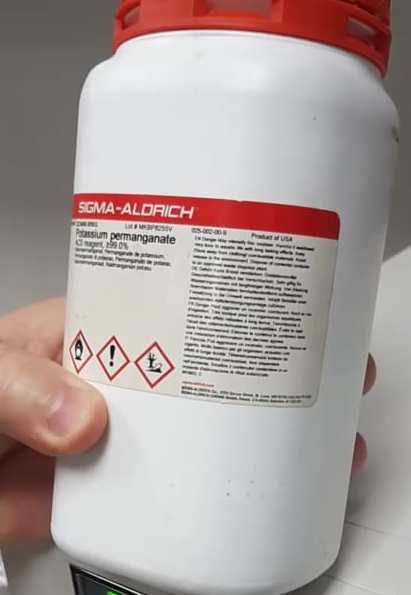
\includegraphics[width=0.3\textwidth]{Tarea1/muestras.png}
    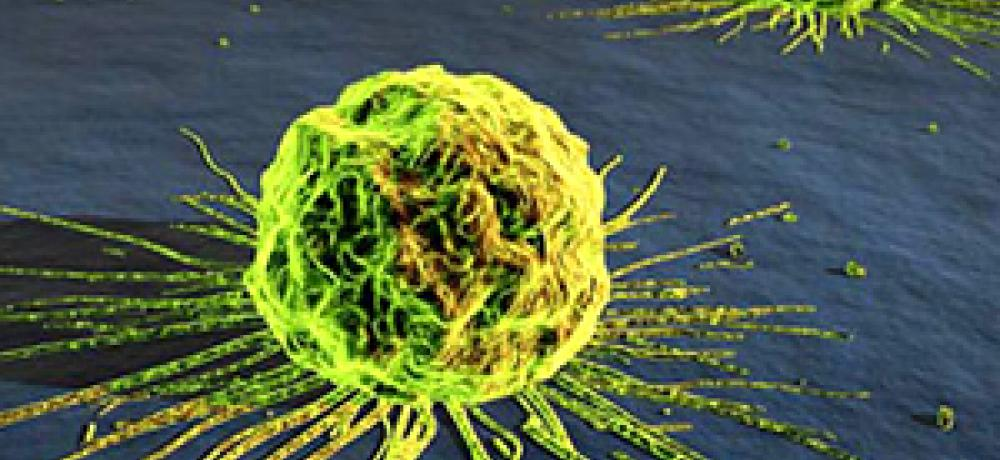
\includegraphics[width=0.49\textwidth]{Tarea5/nano.png}
    \caption{\textbf{Nanodiamantes presentados en la revista de Science Translational Medicine.}}
    \label{nano}
\end{figure}

Actualmente ya es posible por los científicos crear una combinación de fármaco y nanodiamante que puede ser inyectado en los tumores, consiguiendo así una mayor retención del químico en el interior del tumor y por ende un aumento de la eficacia del tratamiento sin afectar a los tejidos cercanos y de esta forma reducir los efectos tóxicos derivados de la quimioterapia. Esto presenta un gran avance en los tratamientos actuales ya que los tumores de manera general son difíciles de tratar debido a que los fármacos de la quimioterapia inyectados son incapaces de penetrar en ciertas partes del sistema de protección de vasos sanguíneos (ejemplo de este es el que rodea el cerebro). 



Este hallazgo demuestra que la colaboración entre bioingeniería y medicina es fundamental para desarrollar un futuro tratamiento menos nocivo y más contundente contra la enfermedad.

\textbf{Conteo de celulas en una cámara de Neubauer.}

La cámara de Neubauer es un instrumento utilizado en medicina y biología para realizar el recuento de esporas y células en un medio líquido, que puede ser; un cultivo celular, sangre, orina, líquido cefalorraquídeo, líquido sinovial, etc.

La misma tradicionalmente está adaptada al microscopio (Fig. \ref{microscopio}), ella tiene forma de un portaobjetos que tiene dos zonas ligeramente deprimidas en cuyo fondo se ha marcado con la ayuda de un diamante una cuadrícula de dimensiones conocidas. Se cubre la cámara con un cubreobjetos que se adhiere por simple tensión superficial (en especial una vez que se haya añadido la muestra líquida).

Luego se introduce por capilaridad entre la cámara y el cubre, el líquido con las células a contar, generalmente tras una dilución previa; la cámara tiene dos zonas lo que permite hacer dos recuentos simultáneamente. Se observa la retícula al microscopio con el aumento adecuado y se cuentan las células.

A partir del número de células contadas, conociendo el volumen de líquido que admite el campo de la retícula, se cálcula la concentración de células en la muestra líquida aplicada. El cálculo de la concentración de células se puede expresar así:
\begin{equation}
    \label{concentracion}
    C_T = \dfrac{C_o}{(A)\cdot (h) }\cdot \delta
\end{equation}
donde $C_T$ es la concentracion por mililitros cúbicos, $C_o$ conteo de partículas, $A$ es el área de la camara de conteo, $h$ profundidad de la cámara y $\delta$ es la dilución.

En la retícula central, la cámara de Neubauer tiene un cuadrado primario que contiene nueve cuadrados secundarios, cada uno de ellos dividido a su vez en 16 cuadrados terciarios. El cuadrado secundario central contiene no 16, sino 25 cuadrados, cada uno de ellos dividido a su vez en 16 cuadrados cuaternarios. En los bordes de este cuadrado central se cuentan los hematíes, utilizando sólo los cuadrados de los bordes del terciario central y uno de los centrales. En los secundarios de los bordes superiores e inferiores de la cámara se hace el recuento leucocitario.


\textbf{Estudios de Toxicidad de nanodiamentes con el espectrofotómetro.}

Otro problema muy común en el área de producción es que cuando se diseña y sintetiza un material nuevo, con el objetivo de estudiar su comportamiento para alguna aplicación futura, como parte del proceso de caracterización se precisa estudiar su toxicidad para su posterior producción, manipulación y comercialización ya que pueden provocar daño a nivel fisiológico, esto hace que los estudios en vitro sean un primer acercamiento práctico y rápido.

\textbf{\textcolor{azul50}{Procedimiento Experimental}}

Se análizará la capacidad de toxicidad que posee las nanopartículas sobre células vivas para esto se hizo uso de diferentes sustancias, entre ellas:

\begin{itemize}
    \item \textbf{\textcolor{morado}{RPMI:}} El medio Roswell Park Memorial Institute (en inglés, Roswell Park Memorial Institute medium),el mismo es usado para cultivos celulares. Tradicionalmente, es usado para el cultivo de células humanas o de tejidos aislados como el caso de las arterias mamarias humanas.
    \item \textbf{\textcolor{morado}{T-47D:}} es una línea celular de cáncer de seno humano comúnmente utilizada en la investigación biomédica que involucra la expresión hormonal de células cancerosas.
    %\item \textbf{\textcolor{morado}{MDA:}} es una de las líneas celulares es una de las más utilizadas para el estudio experimental in vitro del cáncer de mama hormono-independiente. Estás células presentan un crecimiento extraordinariamente rápido en medios de cultivo poco enriquecidos. Se utilizan en estudios bioquímicos y genéticos que han contribuido enormemente a la investigación del cáncer de mama y al desarrollo de fármacos para ayudar a combatirlo.
    \item \textbf{\textcolor{morado}{Azul de metileno:}} 
    se utiliza como colorante en las tinciones para la observación en el microscopio, y para teñir resultados en los laboratorios.
    \item \textbf{\textcolor{morado}{Nanopartículas fluorescentes $900174-5ML$:}} se emplean en diversos métodos de imagen y seguimiento para estudiar cómo las células madre se incorporan y regeneran, al implacar está técnica se implantan en las células madre diminutos diamantes y de esta forma las partículas fluorescentes permiten un seguimiento in vivo de las células.
    \item \textbf{\textcolor{morado}{DmSO:}} Dimetil Sulfóxido, este líquido orgánico incoloro de fórmula química $CH_3SOCH_3$ que contiene sulfóxido, usado como disolvente orgánico industrial a partir de 1940, es utilizado como criopreservante y como un medicamento, posee la propiedad de atravesar rápidamente la epidermis y las membranas celulares, tambien es un disolvente aprótico y altamente polar, por ello, es miscible tanto con el agua como con disolventes orgánicos como alcoholes, cetonas etc. 
\end{itemize}

Primeramente se ralizará el conteo de células para T-47D, para esto se procedió:\\[-1cm]
\begin{itemize}
    \item Se aplicará azúl de tripano en muestras de $T-47D$.
    \item Colocamos las células teñidas en la cámara de Neubauer y realizamos el conteo con el microscopio óptico de la Fig.\ref{microscopio} de las células muertas (coloreadas de azul) y las vivas en los cuadros de control de la cámara.
    \item Se procede al cálculo de las células vivas y muestras por $ml$ haciendo uso de la ec. \ref{concentracion}. 
\end{itemize}

Para valorar la toxicidad de las nanopartículas se procederá con el siguiente experimento:\\[-1cm]
\begin{itemize}
    \item Ya con el valor de $C_T$ obtenido del experimento anterior, se colocan $100\mu l$ del cultivo celular con RPMI en nuestra microplaca.
    \item Se mezclan con los nanodiamantes fluorescentes de forma de que las proporciones sean semejantes a las utilizadas en el procedimiento (B) de la práctica 2 (seccion de obtención de datos).
    \item Se deja repozar hasta el día siguiente, retiramos los nanodiamantes lavando 2 veces con $200~\mu l$ de solución salina y añadimos $100~ \mu l$ de solución RPMI con MTT.
    \item Se deja 30 minutos en incubadora. Retiramos MTT de todas las celdas. Agregamos $50 ~\mu l$ de DmSO en el portamuestras para disolver.
    \item Los resultados de la microplaca se valoraran con el espectrofotómetro de haz monocromático a $570~ nm$.
\end{itemize}

\textbf{\textcolor{azul50}{Análisis de Resultados}}

Al implementar el procedimiento con la camará de Neubauer para una muestra de $T-47D$ se obtuvieron los resultados mostrados en la Fig. \ref{conteo}.
\begin{figure}
    %\centering
    %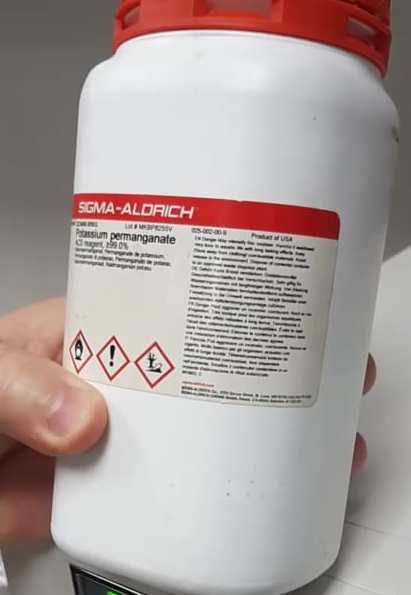
\includegraphics[width=0.3\textwidth]{Tarea1/muestras.png}
    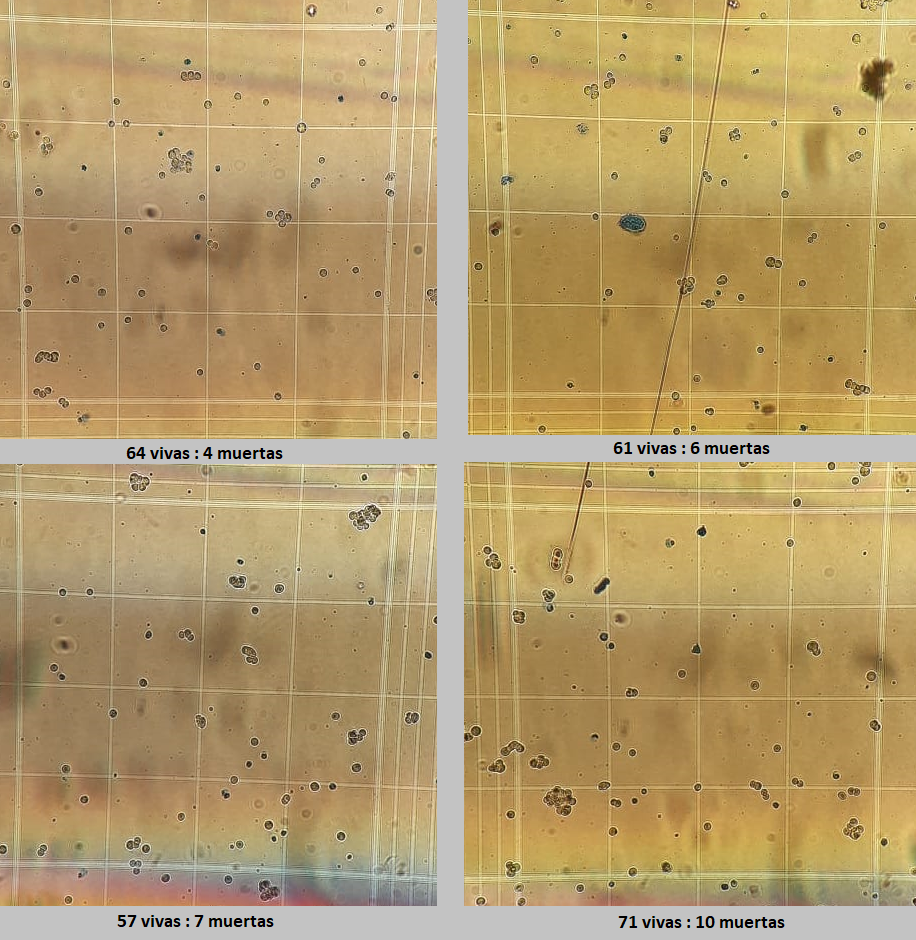
\includegraphics[width=0.39\textwidth]{Tarea5/conteo.png}
    \caption{\textbf{imagenes obtenidas por el microscopio electrónico.}}
    \label{conteo}
\end{figure}
Se puede concluir que entre $6.3\% - 14.3\%$ de las células estaban muertas. Resultado de la implementación de la ec. \ref{concentracion} tenemos que $C_T\approx (15.8 \pm 1.5)\cdot 10^6 ~~cell/ml$, para células vivas. Al obtener y gráficar los resultados reportados por el espectrofotómetro, obtenemos los resultados mostrados en la Fig. \ref{toxicidad}.

El gráfico muestra cambios en la presencia de cristales formados en nuestra muestra, de aquí se puede concluir que si hay efectos de toxicidad visibles como resultado de la presencia de las nanopartículas en nuestra muestra, un análisis de ajuste no fue considerado ya que existe mucha dispersión en los valores obtenidos y existen pocos casos tratados como para considerarlo.
\begin{figure}
    %\centering
    %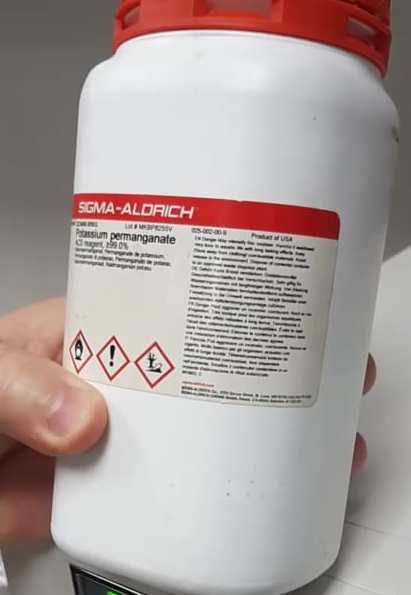
\includegraphics[width=0.3\textwidth]{Tarea1/muestras.png}
    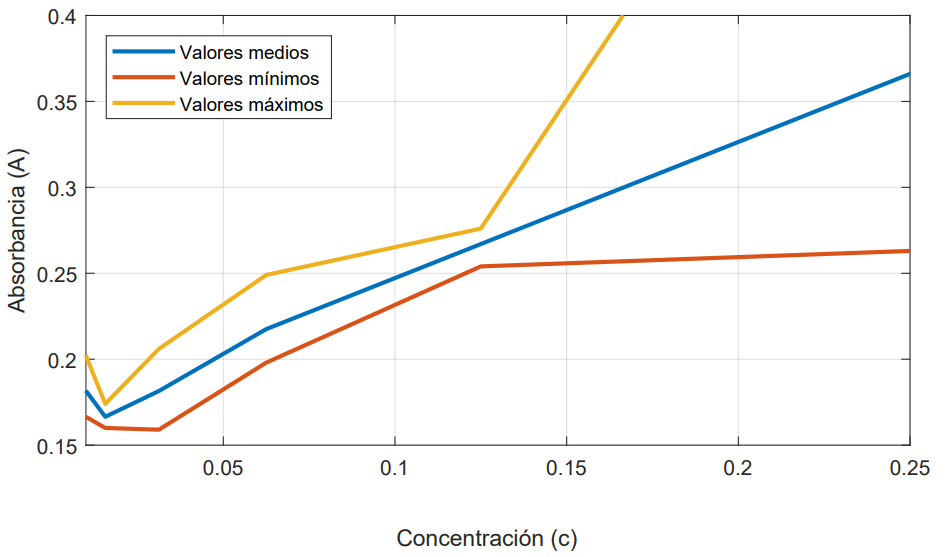
\includegraphics[width=0.49\textwidth]{Tarea5/nano_con_cell.png}
    \caption{\textbf{Procesamiento de los valores de Absorbancia.}}
    \label{toxicidad}
\end{figure}



\textbf{\textcolor{azul50}{Conclusiones}}

El objetivo del laboratorio fue cumplido mediante el conteo utilizando la cámara de Neubauer y al realizar el respectivo análisis de muestras celulares, se comprobó que las nanopartículas si poseen un efecto de toxicidad, no se logró profundizar por la falta de datos, con esto se cumple el objetivo del laboratorio.


%\section{Desarrollo}
%\subsection{Generalización para el cálculo CPA con total aleatoriedad espacial}% con $i$ direcciones espaciales.}

%\input{Trabajo/Trabajo.tex}
%\section{Conclusiones}
%\input{Conclusiones/Conclusiones.tex}

%\input{antiguo.tex}
%\section{Agradecimientos}
%\input{Agradecimientos/Agradecimientos.tex}

%\bibliographystyle{ieeetr}
%\renewcommand{\bibname}{Referencias}
% \bibliography{bibliografia/bibliografia}
% \addcontentsline{toc}{chapter}{Referencias Bibliogr\'aficas}

%% For BibTeX users

%\bibliographystyle{rcfbib}
%\bibliography{path}


\end{document}
